\documentclass[a4paper,11pt,abstracton,hidelinks]{scrartcl}

\usepackage[margin=3cm]{geometry}
\usepackage{graphicx}
\usepackage[UKenglish]{babel}
\usepackage{csquotes}
\usepackage[style=numeric,citestyle=numeric,backend=biber,sorting=none,doi=false,url=false]{biblatex}
\usepackage{float}
\usepackage[export]{adjustbox}
\usepackage[T1]{fontenc}
\usepackage{lmodern}
\usepackage[textsize=tiny]{todonotes}
\usepackage[labelsep=period,font=small,labelfont=bf,format=plain]{caption}
\captionsetup[table]{
  position=above,
  belowskip=10pt,
  aboveskip=0pt,
}
\usepackage[group-separator={,}]{siunitx}
\usepackage{booktabs}
\usepackage{pdflscape}
\usepackage{tablefootnote}
\usepackage{authblk}
\usepackage{threeparttable}
\usepackage{afterpage}
\usepackage{lineno}
\linenumbers
\usepackage{setspace}
\usepackage{hyperref}
\doublespacing

\newcommand{\beginsupplement}{%
  \setcounter{table}{0}
  \renewcommand{\thetable}{S\arabic{table}}%
  \setcounter{figure}{0}
  \renewcommand{\thefigure}{S\arabic{figure}}%
}


\addbibresource{refs.bib}


\title{
The genetic architecture of target-site resistance to pyrethroid insecticides in the African malaria vectors \emph{Anopheles gambiae} and \emph{Anopheles coluzzii}
}


\author[1]{Chris S. Clarkson}
\author[2,1]{Alistair Miles}
\author[2]{Nicholas J. Harding}
\author[1,2]{Dominic Kwiatkowski}
\author[3,1]{Martin Donnelly}
\author[4]{The \emph{Anopheles gambiae} 1000 Genomes Consortium}
\affil[1]{Wellcome Trust Sanger Institute, Hinxton, Cambridge CB10 1SA}
\affil[2]{Big Data Institute, Old Road, Oxford OX3 7FZ}
\affil[3]{Liverpool School of Tropical Medicine, Pembroke Place, Liverpool L3 5QA}
\affil[4]{https://www.malariagen.net/projects/ag1000g\#people}

\begin{document}


\maketitle


\begin{abstract}


%%
Resistance to pyrethroid insecticides is a major concern for malaria vector control, because these are the only compounds approved for use in insecticide-treated bed-nets (ITNs), and are also widely used for indoor residual spraying (IRS). 
%
Pyrethroids target the voltage-gated sodium channel (VGSC) protein, an essential component of the mosquito nervous system, but substitutions in the amino acid sequence can disrupt the activity of these insecticides, inducing a resistance phenotype. 
%
Here we use Illumina whole-genome sequence data from phase 1 of the \emph{Anopheles gambiae} 1000 Genomes Project (Ag1000G) to provide a comprehensive account of genetic variation at the \emph{Vgsc} locus in mosquito populations from 8 African countries.
%
In addition to the three known resistance alleles, we describe 20 non-synonymous nucleotide substitutions at appreciable frequency in one or more populations that are previously unknown in mosquitoes.
%
We analyse the genetic backgrounds on which known and putative resistance alleles are found, to determine which alleles have experienced recent positive selection, and to refine our understanding of the origins and spread of resistance between species and geographical locations.
%
We identify ten distinct haplotype clusters under selection, five of which carry the L995F resistance allele, four of which carry L995S, and one of which carries I1527T.
%
Five of these clusters are localised to a single geographical location, and five comprise haplotypes from two or more countries, indicating the geographical spread of resistance.
%
We also find evidence for multiple introgression events transmitting resistance alleles between the two mosquito species.
%
For each novel variant allele we predict a putative resistance phenotype based on genetic evidence for positive selection, patterns of genetic linkage between variants, location of the variant within the protein domain architecture, and functional evidence from other species.
%
Thirteen of these novel alleles occur almost exclusively on haplotypes carrying the known L995F resistance allele, and appear to be secondary mutations that may enhance or compensate for the L995F resistance phenotype.
%
The I1527T substitution, which is adjacent to a predicted pyrethroid binding site in the channel molecule, occurs in tight linkage with either of two alleles causing a V402L substitution, orthologous to a combination of substitutions found to cause pyrethroid resistance in several other insect species.
%
Our results demonstrate that the molecular basis of pyrethroid resistance in African malaria vectors is more complex than previously appreciated, and provide a foundation for the design of new genetic tools to track the spread insecticide resistance and to inform vector control.
%%

\end{abstract}


\section*{Introduction}


%%
Pyrethroid insecticides have been the cornerstone of malaria prevention in Africa for almost two decades \cite{Bhatt2015}.
%
Pyrethroids are still the only class of insecticide approved for use in insecticide-treated bed-nets (ITNs), and are widely used in indoor residual spraying (IRS) campaigns as well as in agriculture.
%
Pyrethroid resistance is, however, now widespread in malaria vector populations across Africa \cite{Hemingway2016}.
%
The World Health Organisation (WHO) has published plans for insecticide resistance management (IRM), which emphasise the need for improvements in our ability to monitor resistance, and for improvements in our understanding of the molecular mechanisms of resistance \cite{WorldHealthOrganization2012}.
%%


%%
The voltage-gated sodium channel (VGSC) is the physiological target of pyrethroid insecticides, and is integral to the insect nervous system. 
%
Pyrethroid molecules bind to sites within the protein channel and prevent normal nerve function, causing paralysis (``knock-down'') and then death. 
%
However, amino acid substitutions at key positions within the protein alter the interaction with insecticide molecules, increasing the dose of insecticide required for knock-down (target-site resistance) \cite{Davies2007a}. 
%
In the African malaria vectors \textit{Anopheles gambiae} and \textit{An. coluzzii}, three substitutions have been found to cause pyrethroid resistance. 
%
Two of these substitutions occur in codon 995\footnotemark, with \texttt{L995F} prevalent in West and Central Africa \cite{Martinez-Torres1998,Silva2014}, and \texttt{L995S} found in Central and East Africa \cite{Ranson2000,Silva2014}. 
%
\footnotetext{Codon numbering is given here relative to transcript AGAP004707-RA as defined in the AgamP4.4 gene annotations. A mapping of codon numbers from AGAP004707-RA to \emph{Musca domestica}, the system in which the \emph{kdr} mutations were first discovered \cite{Williamson1996}, is given in Table 1 and in @@Supplementary data.}
%
A third substitution, \texttt{N1570Y}, has been found in Central Africa and shown to increase resistance in association with \texttt{L995F} \cite{Jones2012}.
%
However, studies in other insect species have found a variety of other \emph{Vgsc} substitutions inducing a resistance phenotype \cite{Davies2007b,Rinkevich2013,Dong2014}. 
%
To our knowledge, no studies in malaria vectors have analysed the full \emph{Vgsc} coding sequence, thus the molecular basis of target-site resistance to pyrethroids has not been fully explored.
%%


%%
Basic information is also lacking about the origins and spread of pyrethroid resistance in malaria vectors. 	
%
For example, it is not known when, where or how many times pyrethroid target-site resistance has emerged. 
%
The paths of transmission, carrying resistance alleles between mosquito populations, are also not known. 
%
Previous studies have found evidence that \texttt{L995F} occurs on several different genetic backgrounds, suggesting multiple independent outbreaks of resistance driven by this allele \cite{Pinto2007,Etang2009,Santolamazza2015}. 
%
However, these studies analysed only a small gene region in a limited number of mosquito populations, and therefore had limited resolution to make inferences about genetic relationships between gene sequences (haplotypes) carrying this allele. 
%
It has also been shown that the \texttt{L995F} allele spread from \textit{An. gambiae} to \textit{An. coluzzii} in West Africa \cite{Clarkson2014,Norris2015}. 
%
However, both \texttt{L995F} and \texttt{L995S} now have wide geographical distributions \cite{Silva2014}, and no attempts have been made to infer or track the geographical spread of either allele.
%%

%%
Here we report an in-depth analysis of the VGSC gene, using whole-genome Illumina sequence data from phase 1 of the \emph{Anopheles gambiae} 1000 Genomes Project (Ag1000G) \cite{Ag1000gConsortium2017}.
%
The Ag1000G phase 1 resource includes data on nucleotide variation in 765 wild-caught mosquitoes sampled from 8 countries, with representation of West, Central and East Africa, and of both \textit{An. gambiae} and \textit{An. coluzzii}.
%
We investigate variation across the complete gene coding sequence, and report population genetic data for both known and novel non-synonymous nucleotide substitutions.
%
We then use haplotype data from the chromosomal region spanning the VGSC gene to study the genetic backgrounds carrying resistance alleles, and infer the geographical spread of resistance between mosquito populations.
%
Finally, we explore ways in which variation data from Ag1000G could be used to design high-throughput, low-cost genetic assays for monitoring pyrethroid resistance, with the capability to differentiate and track separate resistance outbreaks.  
%%


%%%%%%%%%%%%%%%%%%%%%%%%%%%%%%%%%%%%%%%%%%%%%%%%%%%%%%%%%%%%%%%%%%%%%%%%%%%%%%%
%%%%%%%%%%%%%%%%%%%%%%%%%%%%%%%%%%%%%%%%%%%%%%%%%%%%%%%%%%%%%%%%%%%%%%%%%%%%%%%


\section*{Results}


%%%%%%%%%%%%%%%%%%%%%%%%%%%%%%%%%%%%%%%%%%%%%%%%%%%%%%%%%%%%%%%%%%%%%%%%%%%%%%%
\subsection*{\textit{Vgsc} non-synonymous nucleotide variation}


%% Paragraph 1
%
To identify variants with a potentially functional role in pyrethroid resistance, we extracted single nucleotide polymorphisms (SNPs) that alter the amino acid sequence of the VGSC protein from the Ag1000G phase 1 data resource.
%
We then computed their allele frequencies among 9 mosquito populations defined by species and country of origin.
%
Alleles that confer resistance are expected to increase in frequency under selective pressure, and we filtered the list of potentially functional variant alleles to retain only those at or above 5\% frequency in one or more populations (Table \ref{table:variants_missense}).
%
The resulting list comprises 23 variant alleles, including the known \texttt{L995F}, \texttt{L995S} and \texttt{N1570Y} resistance alleles, and a further 20 alleles not previously described in these species.
%
We reported 15 of these novel alleles in our global analysis of the Ag1000G phase 1 data resource \cite{Ag1000gConsortium2017}, and we extend the analyses here to incorporate a SNP which alters codon 1603 and two tri-allelic SNPs affecting codons 402 and 490.
%%


%% Table 1 - Functional SNPs.
%
\afterpage{%
%\clearpage
% N.B., for some reason using \newgeometry causes page number to get dropped from the subsequent page, so disable for now - not needed if using \footnotesize.
%\newgeometry{margin=2cm}
%\begin{landscape}
\thispagestyle{empty}
\begin{table}[h]
  \scriptsize
  %\centering
  \begin{threeparttable}

  \caption{
%
\textbf{Non-synonymous nucleotide variation in the voltage-gated sodium channel gene}. 
%
AO=Angola; BF=Burkina Faso; GN=Guinea; CM=Cameroon; GA=Gabon; UG=Uganda; KE=Kenya; GW=Guinea-Bissau; \textit{Ac}=\textit{An. coluzzii}; \textit{Ag}=\textit{An. gambiae}.
%
All variants are at 5\% frequency or above in one or more of the 9 Ag1000G phase 1 populations, with the exception of \texttt{2,400,071 G>T} which is only found in the CM\emph{Ag} population at 0.4\% frequency but is included because another mutation (\texttt{2,400,071 G>A}) is found at the same position causing the same amino acid substitution (\texttt{M490I}); and \texttt{2,431,019 T>C} (\texttt{F1920S}) which is at 4\% frequency in GA\emph{Ag} but also found in CM\emph{Ag} and linked to \texttt{L995F}. 
}

  \label{table:variants_missense}
  
  
\begin{tabular}{lllrrrrrrrrrrr}
\toprule
\multicolumn{3}{c}{Mutation} &
\multicolumn{9}{c}{Population allele frequency (\%)} &
\multicolumn{2}{c}{LD ($D'$)} \\
\cmidrule(r){1-3}
\cmidrule(r){4-12}
\cmidrule(r){13-14}
Position\tablefootnote{Position relative to AgamP3 reference sequence, chromosome arm 2L.} & 
\emph{Ag}\tablefootnote{Codon numbering according to transcript \texttt{AGAP004707-RA} in geneset AgamP4.4.} & 
\emph{Md}\tablefootnote{Codon numbering according to \emph{Musca domestica Vgsc} EMBL accession X96668 \cite{williamson1996}.} & 
AO\emph{Ac} & 
BF\emph{Ac} & 
GN\emph{Ag} & 
BF\emph{Ag} & 
CM\emph{Ag} & 
GA\emph{Ag} & 
UG\emph{Ag} & 
KE & 
GW & 
\texttt{L995S} & 
\texttt{L995F} \\
\midrule

\texttt{2,390,177 G>A} & \texttt{R254K} & \texttt{R261} & 0 & 0 & 0 & 0 & 32 & 21 & 0 & 0 & 0 & -0.98 & 0.96 \\

\texttt{2,391,228 G>C} & \texttt{V402L} & \texttt{V410} & 0 & 7 & 0 & 0 & 0 & 0 & 0 & 0 & 0 & -1 & -0.41 \\

\texttt{2,391,228 G>T} & \texttt{V402L} & \texttt{V410} & 0 & 7 & 0 & 0 & 0 & 0 & 0 & 0 & 0 & -1 & 0.10 \\

\texttt{2,399,997 G>C} & \texttt{D466H} & \texttt{-} & 0 & 0 & 0 & 0 & 7 & 0 & 0 & 0 & 0 & -1 & 1 \\

\texttt{2,400,071 G>A} & \texttt{M490I} & \texttt{M508} & 0 & 0 & 0 & 0 & 0 & 0 & 0 & 18 & 0 & -0.33 & -1 \\

\texttt{2,400,071 G>T} & \texttt{M490I} & \texttt{M508} & 0 & 0 & 0 & 0 & 0 & 0 & 0 & 0 & 0 & -1 & -0.01 \\

\texttt{2,416,980 C>T} & \texttt{T791M} & \texttt{T810} & 0 & 1 & 13 & 14 & 0 & 0 & 0 & 0 & 0 & -1 & 1 \\

\texttt{2,422,651 T>C} & \texttt{L995S} & \texttt{L1014} & 0 & 0 & 0 & 0 & 15 & 64 & 100 & 76 & 0 & 1 & -1 \\

\texttt{2,422,652 A>T} & \texttt{L995F} & \texttt{L1014} & 86 & 85 & 100 & 100 & 53 & 36 & 0 & 0 & 0 & -1 & 1 \\

\texttt{2,424,384 C>T} & \texttt{A1125V} & \texttt{K1133} & 9 & 0 & 0 & 0 & 0 & 0 & 0 & 0 & 0 & -1 & -1 \\

\texttt{2,425,077 G>A} & \texttt{V1254I} & \texttt{I1262} & 0 & 0 & 0 & 0 & 0 & 0 & 0 & 0 & 5 & -1 & -1 \\

\texttt{2,429,617 T>C} & \texttt{I1527T} & \texttt{I1532} & 0 & 14 & 0 & 0 & 0 & 0 & 0 & 0 & 0 & -1 & -1 \\

\texttt{2,429,745 A>T*} & \texttt{N1570Y} & \texttt{N1575} & 0 & 26 & 10 & 22 & 6 & 0 & 0 & 0 & 0 & -1 & 0.98 \\

\texttt{2,429,897 A>G} & \texttt{E1597G} & \texttt{E1602} & 0 & 0 & 6 & 4 & 0 & 0 & 0 & 0 & 0 & -1 & 1 \\

\texttt{2,429,915 A>C} & \texttt{K1603T} & \texttt{K1608} & 0 & 5 & 0 & 0 & 0 & 0 & 0 & 0 & 0 & -1 & 1 \\

\texttt{2,430,424 G>T} & \texttt{A1746S} & \texttt{A1751} & 0 & 0 & 11 & 13 & 0 & 0 & 0 & 0 & 0 & -1 & 1 \\

\texttt{2,430,817 G>A} & \texttt{V1853I} & \texttt{V1858} & 0 & 0 & 8 & 5 & 0 & 0 & 0 & 0 & 0 & -1 & 1 \\

\texttt{2,430,863 T>C} & \texttt{I1868T} & \texttt{I1873} & 0 & 0 & 18 & 25 & 0 & 0 & 0 & 0 & 0 & -1 & 1 \\

\texttt{2,430,880 C>T} & \texttt{P1874S} & \texttt{P1879} & 0 & 21 & 0 & 0 & 0 & 0 & 0 & 0 & 0 & -1 & 1 \\

\texttt{2,430,881 C>T} & \texttt{P1874L} & \texttt{P1879} & 0 & 7 & 45 & 26 & 0 & 0 & 0 & 0 & 0 & -1 & 1 \\

\texttt{2,431,061 C>T} & \texttt{A1934V} & \texttt{A1939} & 0 & 12 & 0 & 0 & 0 & 0 & 0 & 0 & 0 & -1 & 1 \\

\texttt{2,431,079 T>C} & \texttt{I1940T} & \texttt{I1945} & 0 & 4 & 0 & 0 & 7 & 0 & 0 & 0 & 0 & -1 & 1 \\

\bottomrule
\end{tabular}


  \begin{tablenotes}
    \footnotesize
    
    \item[1] Position relative to the AgamP3 reference sequence, chromosome arm 2L. Variants marked with an asterisk (*) failed conservative variant filters applied genome-wide in the Ag1000G phase 1 AR3 callset, but appeared sound on manual inspection of read alignments.
    
    \item[2] Codon numbering according to \emph{Anopheles gambiae} transcript AGAP004707-RA in geneset AgamP4.4.
    
    \item[3] Codon numbering according to \emph{Musca domestica} EMBL accession X96668 \cite{Williamson1996}.
    
  \end{tablenotes}
  
  \end{threeparttable}
  
\end{table}
%\end{landscape}
%\restoregeometry
} % end afterpage
%% end Table 1


%% L995F, L995S
The two known resistance alleles affecting codon 995 had the highest overall allele frequencies within the Ag1000G phase 1 cohort.
%
The \texttt{L995F} allele was at high frequency in populations of both species from West, Central and Southern Africa.
%
The \texttt{L995S} allele was at high frequency among \textit{An. gambiae} populations from Central and East Africa.
%
Both alleles were present in \textit{An. gambiae} populations sampled from Cameroon and Gabon, including some individuals with a hybrid \texttt{L995F/S} genotype (46/275 individuals in Cameroon, 36/56 in Gabon).
%
In Cameroon these alleles were in Hardy Weinberg equilibrium ($\chi^{2}$ = 0.02, P > 0.05), thus there does not appear to be selection for or against heterozygote carriers of both alleles.
%
However, there was an excess of heterozygotes in Gabon ($\chi^{2}$ = 8.96, P < 0.005), suggesting a fitness advantage for mosquitoes carrying both alleles.
%%


% I'm not clear on what this is saying, so have commented out for now. I.e., why do we report these data, what do they show? Do they support the hypothesis that the resistance phenotype is incompletely recessive? If so, can we make this clearer?
%289 samples in the dataset carried $\geq$1 \texttt{L995F} alleles of which 92 were homozygotes and in the case of \texttt{L995S}, 156 samples carried $\geq$1 alternative alleles and of these 38 were homozygotes; the resistance phenotype at this locus is thought to be incompletely recessive \cite{Chandre2000}.
%%


%% Figure - Pairwise LD.
%
\begin{figure}[!t]

  \centering
  
  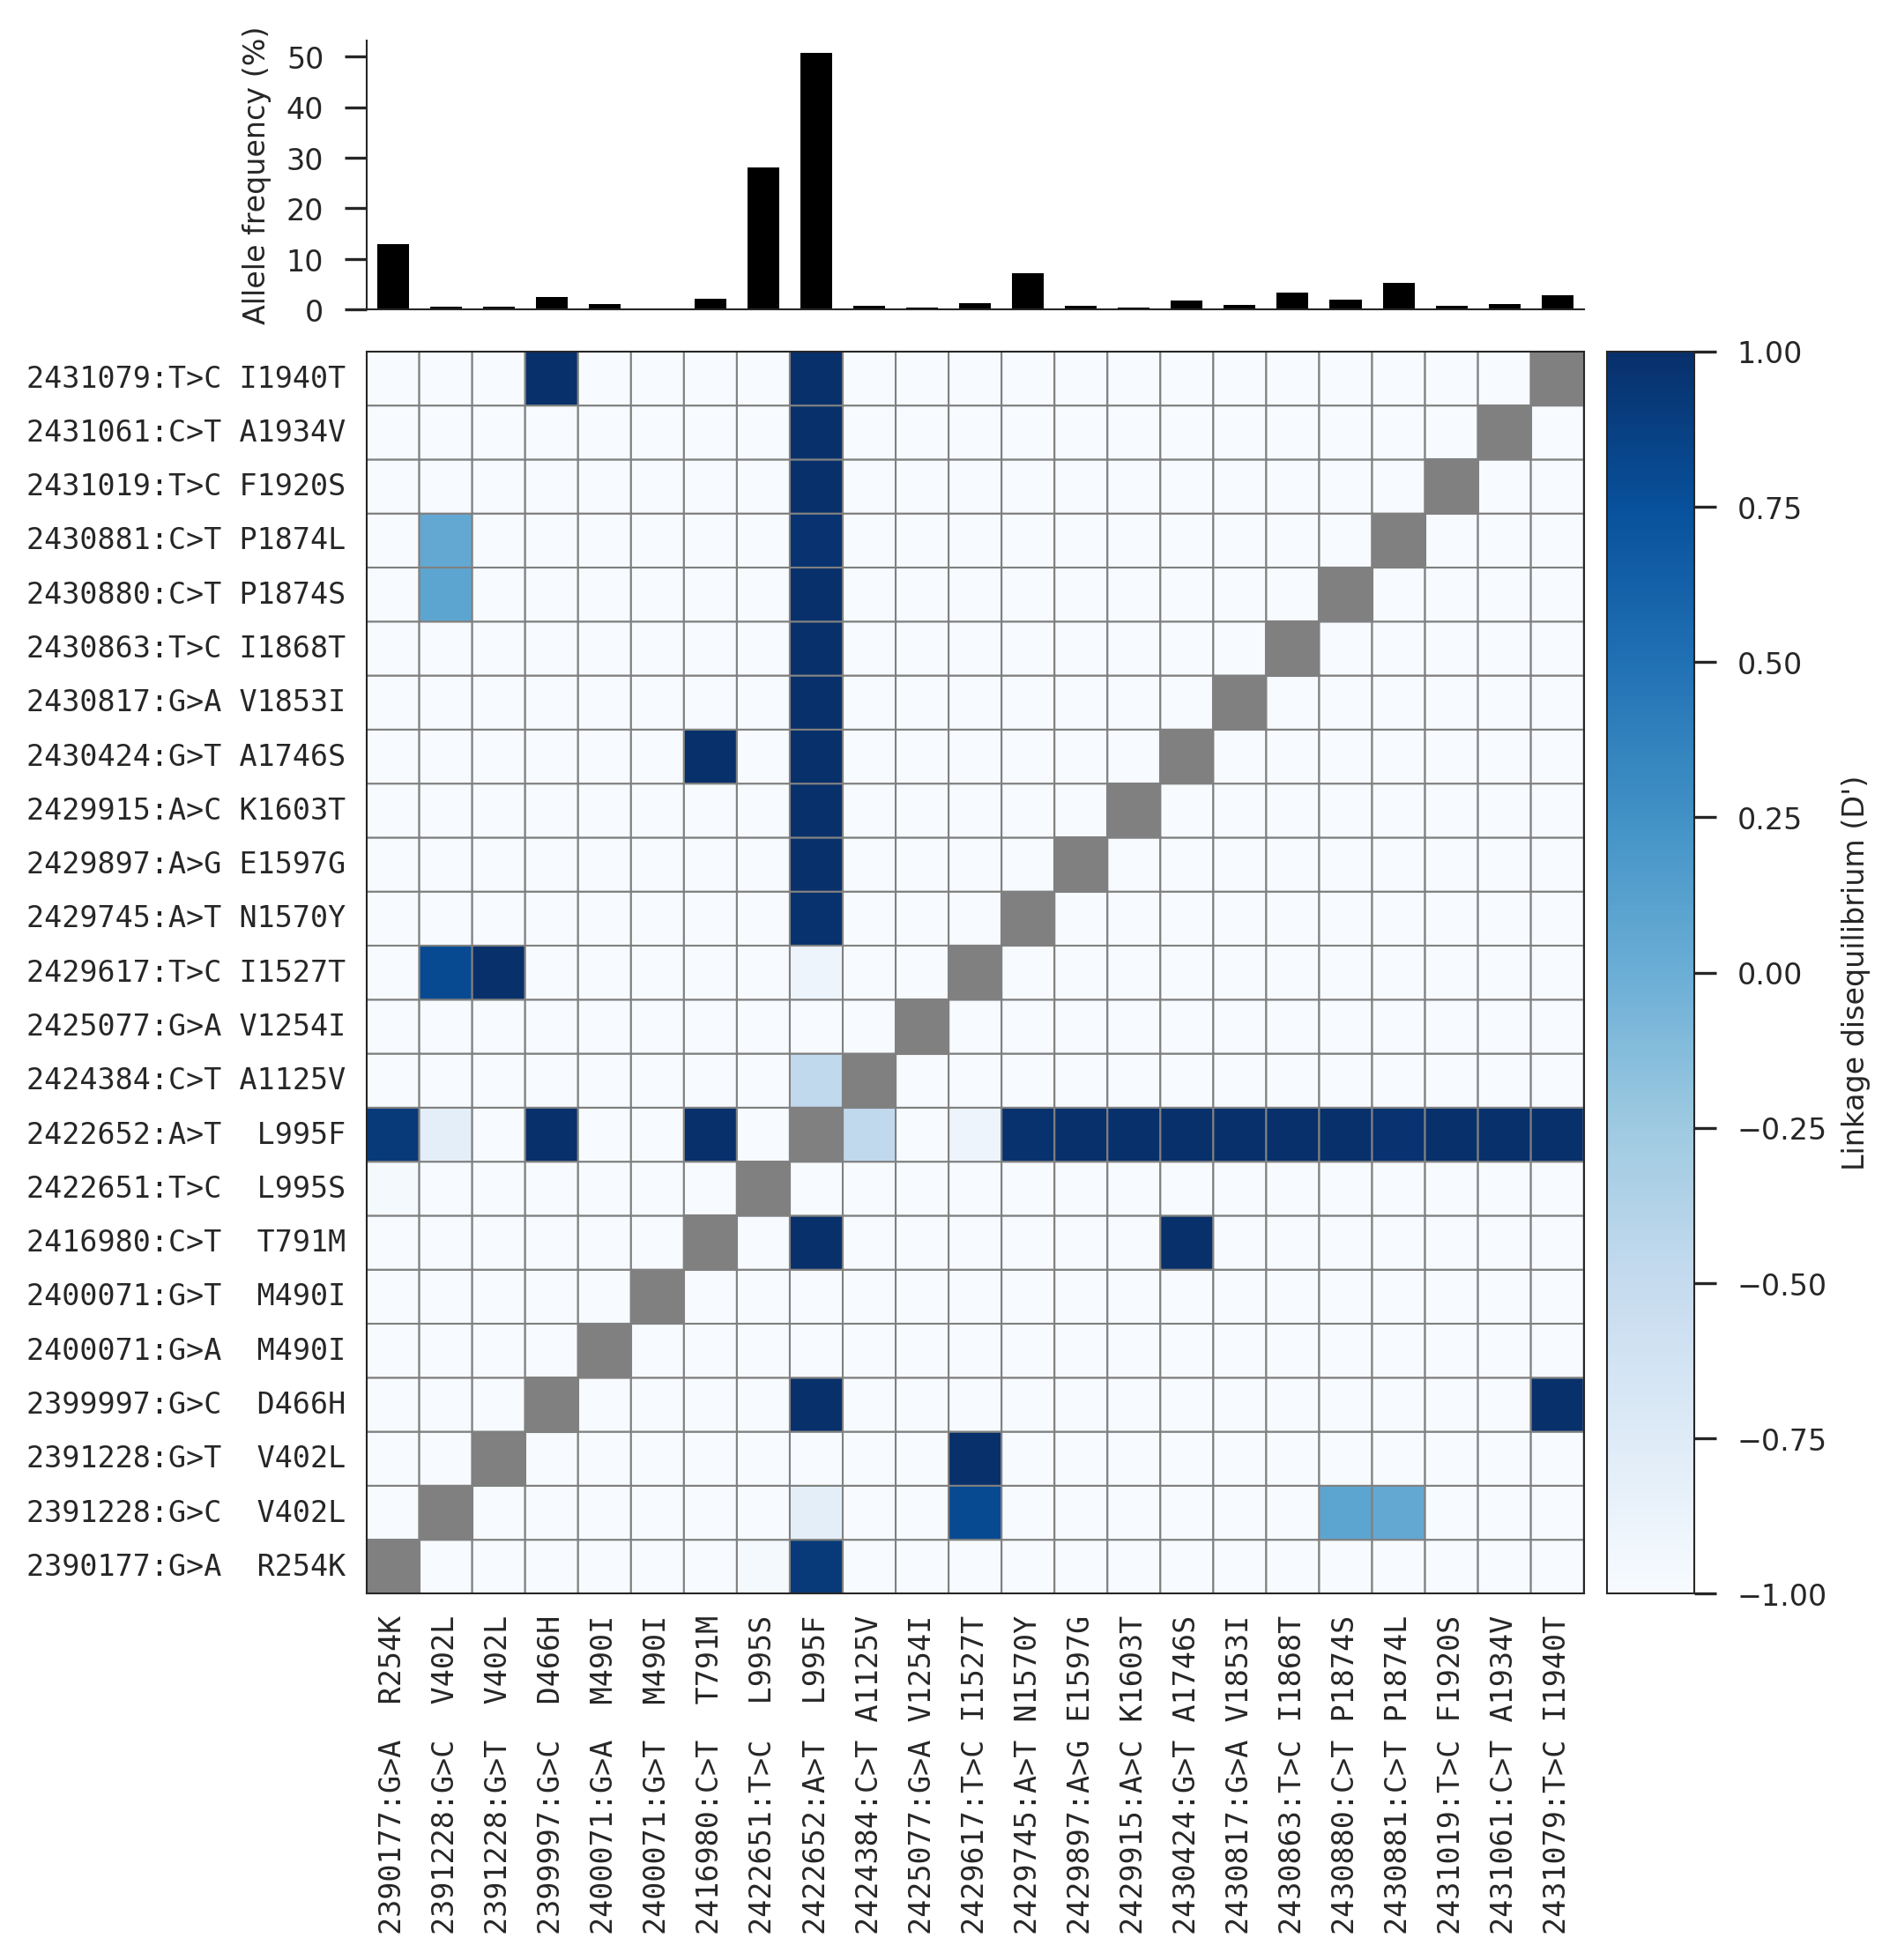
\includegraphics[width=\linewidth]{artwork/fig_ld.png}
  
  \caption{\textbf{Linkage disequilibrium between non-synonymous variants}. A value of 1 indicates that the two alleles are in perfect linkage, meaning that one of the two alleles is only ever found in combination with the other. Conversely, a value of -1 indicates that the two alleles are never found in combination with each other.}
  
  \label{fig:ld}
 
\end{figure}
%%


%% N1570Y
%
The N1570Y resistance variant was present in Guinea, Burkina Faso (both species) and Cameroon.
%
This variant has been shown to increase pyrethroid resistance in \textit{An. gambiae}, however it has only ever been found in association with \texttt{L995F}.
%
Codon 1570 occurs within an internal linker domain of the protein, and so cannot directly affect the binding between pyrethroid molecules and the membrane channel.
%
Thus it has been suggested that \texttt{N1570Y} either enhances or compensates for the \texttt{L995F} phenotype, possibly by altering the channel gating properties \cite{Jones2012}.
%
To study the patterns of association among non-synonymous variants, we used haplotypes from the Ag1000G phase 1 resource to compute the normalised coefficient  of linkage disequilibrium ($D'$) between all pairs of variant alleles (Figure \ref{fig:ld}).
%
As expected, we found \texttt{N1570Y} in almost perfect linkage with \texttt{L995F}, meaning that \texttt{N1570Y} was only ever found on haplotypes also carrying \texttt{L995F}.
%%


%% Novel alleles linked to L995F.
%
Of the 20 novel alleles, 13 also occurred almost exclusively in combination with L995F, exhibiting the same LD pattern as \texttt{N1570Y} (Figure \ref{fig:ld}).
%
These included two variants in codon \texttt{1874} (\texttt{P1874S}, \texttt{P1874L}).
%
\texttt{P1874S} has previously been associated with pyrethroid resistance in the crop pest \textit{Plutella xylostella} \cite{Sonoda2008}.
%
The abundance of high-frequency non-synonymous variants occurring in combination with \texttt{L995F} is striking for two reasons.
%
First, \textit{Vgsc} is a highly conserved gene, expected to be under strong functional constraint and therefore purifying selection, and so any non-synonymous variants should be rare @@REF.
%
Second, in contrast with \texttt{L995F}, we did not observe any high-frequency non-synonymous variants occuring in combination with \texttt{L995S}.
%
This contrast was highly significant when data on all variants within the gene were considered: relative to haplotypes carrying the wild-type \texttt{L995} allele, the ratio of non-synonymous to synonymous nucleotide diversity ($\pi_{N}/\pi_{S}$) was 1.5 (95\% CI [0.8, 2.2]) times higher among haplotypes carrying \texttt{L995S}, but 28.1 (95\% CI [25.2, 31.2]) times higher among haplotypes carrying \texttt{L995F}.
%
These results indicate that \texttt{L995F} has substantially altered the selective regime for other amino acid positions within the protein.
%
A number of secondary substitutions have occurred and risen in frequency, and are likely to be providing some selective advantage in the presence of insecticide pressure.
%%


%% I1527T and V402L.
%
The \texttt{I1527T} allele was present in \textit{An. coluzzii} from Burkina Faso at 14\% frequency.
%
Codon \texttt{1527} occurs within trans-membrane domain segment \texttt{III.S6}, immediately adjacent to a second predicted binding pocket for pyrethroid molecules, thus it is plausible that \texttt{I1527T} could alter pyrethroid binding \cite{Dong2014}.
%
We also found that the two variant alleles affecting codon \texttt{402}, both of which induce a \texttt{V402L} substitution, were in strong linkage with \texttt{I1527T} (D' $\geq$ 0.8; Figure \ref{fig:ld}), and almost all haplotypes carrying \texttt{I1527T} also carried a \texttt{V402L} substitution.
%
The most parsimonious explanation for this pattern of linkage is that the \texttt{I1527T} mutation occurred first, and mutations in codon \texttt{402} subsequently arose on this genetic background or recombined with it.
%
Codon \texttt{402} also occurs within a trans-membrane segment (\texttt{I.S6}), and the \texttt{V402L} substitution has been independently associated with pyrethroid resistance in bedbugs \cite{Yoon2008}.
%
Other substitutions at this codon have also been associated with resistance, \texttt{V402A/G} in the moth crop pests \emph{Helicoverpa zea} \cite{Hopkins2010} and \texttt{V402M} in \emph{Heliothis virescens}, the latter of which has been shown experimentally to confer resistance in \textit{Xenopus} oocytes \cite{Park1997, Lee2013}.
%
@@TODO Aedes combination.
%
Because of the limited geographical distribution of these alleles, we hypothesize that the \texttt{I1527T+V402L} combination represents a pyrethroid resistance allele that arose in West African \textit{An. coluzzii} populations.
%
However, the \texttt{L995F} allele is at higher frequency (85\%) in our Burkina Faso \textit{An. coluzzii} population, and is known to be increasing in frequency \cite{Toe2014}, therefore \texttt{L995F} may provide a stronger resistance phenotype and is thus replacing \texttt{I1527T+V402L}.
%%


%% Other novel variants.
%
The remaining 4 novel alleles (two separate nucleotide substitutions causing \texttt{M490I}; \texttt{A1125V}; \texttt{V1254I}) do not occur in combination with any known resistance allele.
%
All are private to a single population, and (to our knowledge) none have previously been found in other species.
%
All occur within internal linker domains of the protein and are therefore unlikely to directly cause resistance, discussed further below.
%%


%%%%%%%%%%%%%%%%%%%%%%%%%%%%%%%%%%%%%%%%%%%%%%%%%%%%%%%%%%%%%%%%%%%%%%%%%%%%%%%
\subsection*{Genetic backgrounds carrying resistance alleles}

%%
% 
Although it is known that pyrethroid resistance is increasing in prevalence in malaria vector populations across Africa, it has not been clear whether this is being driven by the spread of resistance alleles via gene flow, by resistance alleles emerging independently in multiple locations, or by some combination of both processes.
%
The Ag1000G data resource provides a potentially rich source of information about the spread of insecticide resistance alleles in any given gene, because data are available not only for SNPs in gene coding regions, but also SNPs in introns and flanking intergenic regions, and in neighbouring genes.
%
These additional variants can be used to analyse the genetic backgrounds (haplotypes) on which resistance alleles are found.
%
If mosquitoes from different geographical locations or species carry the same resistance allele on identical or near-identical genetic backgrounds, this implies that the allele has been spread between mosquito populations by the movement and interbreeding of mosquitoes.
%
Conversely, if the same resistance allele is found on different genetic backgrounds in different mosquito populations, this provides evidence that the allele has emerged independently in each population, either because of multiple mutational events since the introduction of pyrethroids, or because the allele was segregating at low frequency prior to the introduction of pyrethroids. 
%%

%%
%
In our global analysis of the Ag1000G phase 1 resource \cite{Ag1000gConsortium2017}, we used 1710 biallelic SNPs from within the 73.5 kbp \textit{Vgsc} gene (@@N exonic, @@N intronic) to compute the number of SNP differences between all pairs of 1530 haplotypes derived from the 765 wild-caught mosquitoes in the phase 1 cohort.
%
We then used the pairwise genetic distances to perform hierarchical clustering, and found that haplotypes carrying resistance alleles in codon \texttt{995} were grouped into 10 distinct clusters of near-identical haplotypes.
%
Five of these clusters carried the \texttt{L995F} allele (labelled F1-F5), and a further five clusters carried \texttt{L995S} (labelled S1-S5).
%
To confirm these initial findings, we used the same haplotype data to construct median-joining networks (Figure \ref{fig:networks}).
%
The network analysis is similar to hierarchical clustering, but allows for the reconstruction and placement of intermediate haplotypes that may not be observed in the data. 
%
It also allows for non-hierarchical relationships between haplotypes, which may arise if recombination events have occured between haplotypes.
%
Furthermore, the visualisation of these networks allows relationships among closely-related haplotypes to be discerned.
%
We constructed these networks up to a maximum edge distance of 2 SNP differences, to ensure that each connected component in the resulting networks captures a collection of closely-related haplotypes.
%
The resulting networks confirmed the presence of 5 distinct groupings of haplotypes carrying \texttt{L995F}, and a further 5 haplotype groups carrying \texttt{L995S}, in close correspondence with the previous results from hierarchical clustering (@@quantify).
%


%% Figure - Haplotype networks.
%
\begin{figure}[!t]
  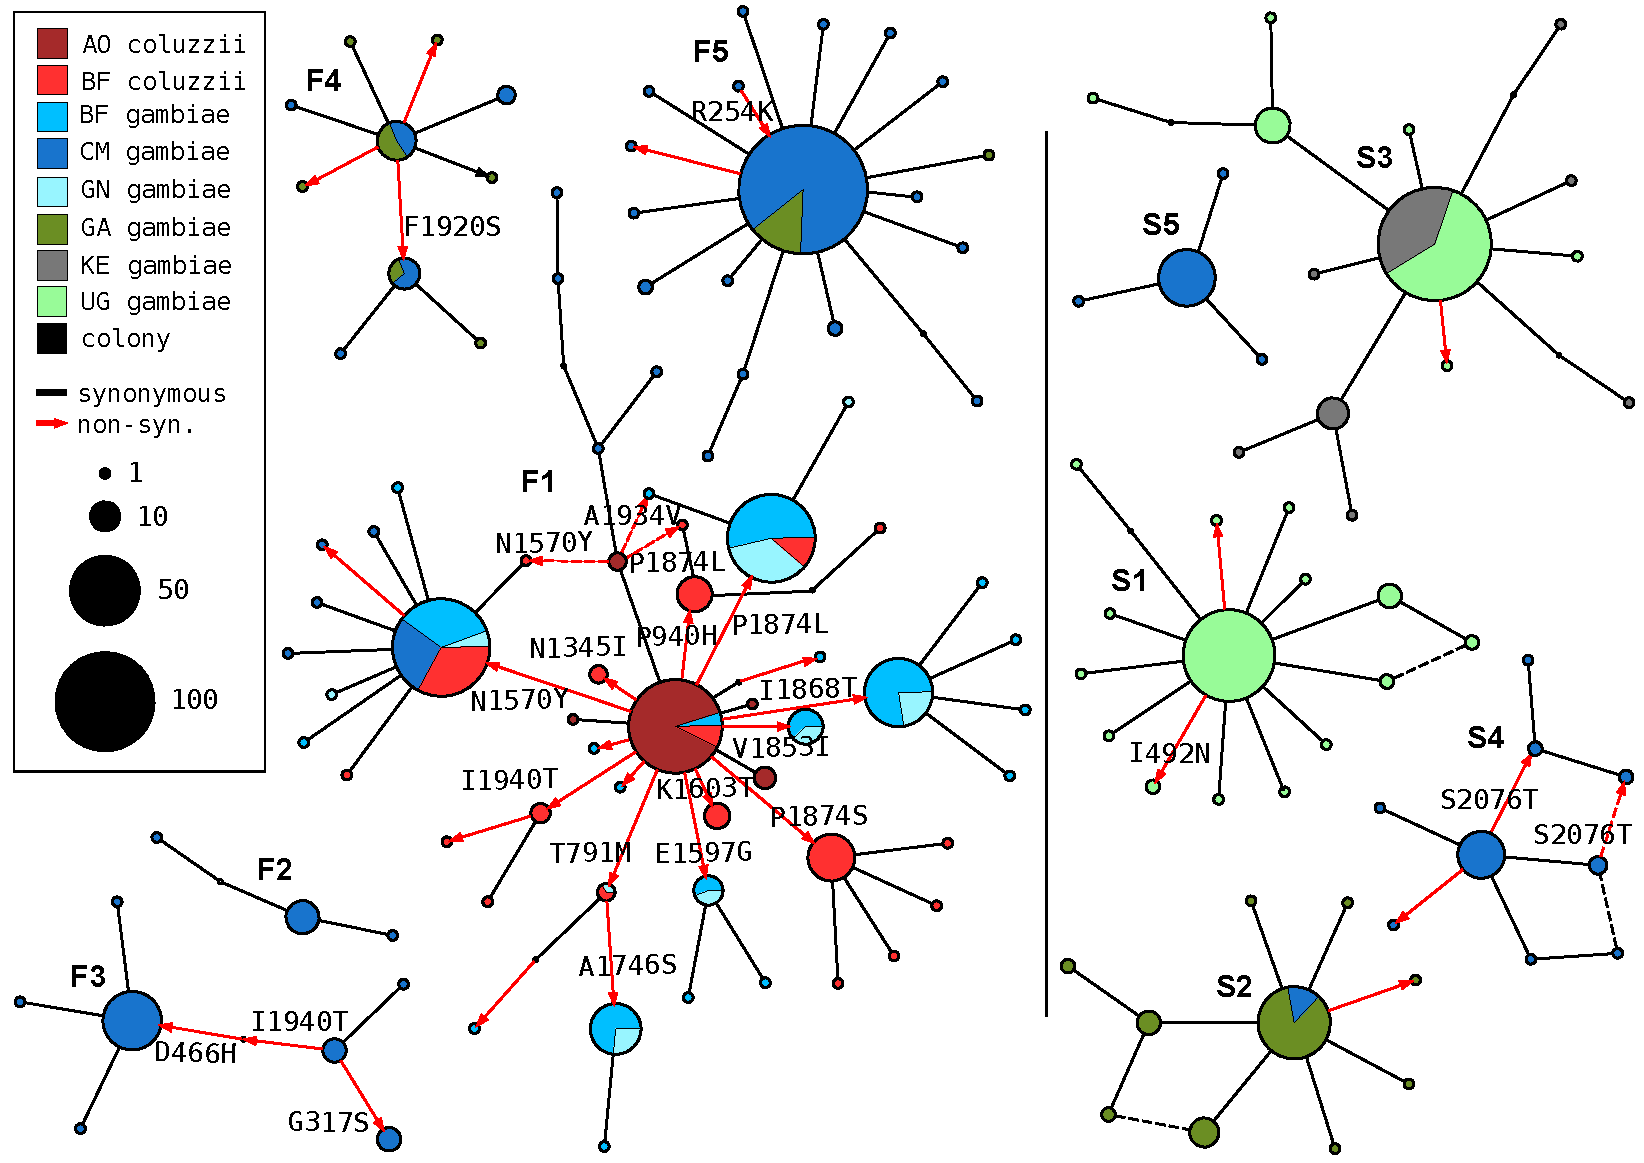
\includegraphics[width=1.1\linewidth,center]{artwork/complete_networks.pdf}
  \caption{\textbf{Haplotype networks}. Median joining networks for haplotypes carrying \texttt{L995F} (labelled F1-F5) or \texttt{L995S} variants (S1-S5) with a maximum edge distance of two SNPs. Network labelling is via concordance with hierarchical clusters discovered in \cite{Ag1000gConsortium2017}. Node size is relative to the number of haplotypes contained and node colour represents the proportion of node haplotypes from mosquito populations/species. Non-synonymous edges are highlighted in red and those leading to non-singleton nodes are labelled with the codon change, arrow head indicates direction of change. Networks consisting of three or more haplotypes are shown.}
  \label{fig:networks}
\end{figure}
%%


%% Observations from the networks.
%
The haplotype networks bring into sharp relief the explosive radiation of amino acid substitutions secondary to the \texttt{L995F} allele.
%
Within the F1 network, nodes carrying non-synonymous variants radiate out from a central node carrying only \texttt{L995F}, suggesting that the central node represents the ancestral haplotype carrying \texttt{L995F} alone which initially came under selection, and these secondary variants have arisen subsequently as new mutations.
%
Many of the nodes carrying secondary variants are large, consistent with positive selection and a functional role for these secondary variants as modifiers of the \texttt{L995F} resistance phenotype (Table \ref{table:variants_pheno}).
%
The F1 network also allows us to infer multiple introgression events between the two species.
%
The central (putatively ancestral) node comprises haplotypes from both species, as do nodes carrying the \texttt{N1570Y}, \texttt{P1874L}, and \texttt{T791M}.
%
This structure is consistent with an initial introgression of the ancestral F1 haplotype, followed later by introgressions of haplotypes carrying secondary mutations.
%
The haplotype networks also illustrate the constrasting levels of non-synonymous variation between \texttt{L995F} and \texttt{L995S}. 
%
Two non-synonymous variants are present within the \texttt{L995S} networks, but both are at low frequency, and thus may be neutral or mildly deleterious variants that are hitch-hiking on selective sweeps for the \texttt{L995S} allele.
%%

%%
%
As well as containing haplotypes from mosquitoes of both species, the F1 network also contains haplotypes from 4 different countries (Guinea, Burkina Faso, Cameroon, Angola).
%
The F4, F5 and S2 networks each contain haplotypes from Cameroon and Gabon.
%
The S3 network contains haplotypes from both Uganda and Kenya.
%
The haplotypes within each of these networks are nearly identical across the entire span of the \textit{Vgsc} gene, and thus it is reasonable to assume that each network captures the descendants of an ancestral haplotype that has risen in frequency due to selection for insecticide resistance and subsequently accumulated other mutations.
%
Given this assumption, these five networks each provide evidence for adaptive gene flow between mosquito populations separated by considerable geographical distances.
%
However, the presence of haplotypes from two different countries within the same network does not imply direct gene flow, as haplotypes could be transmitted from or via a third location, which may be unsampled.
%
%%


%%
%
A limitation of both the hierarchical clustering and network analyses is that they rely on genetic distances within the fixed genomic window from the start to the end of the \textit{Vgsc} gene.
%
\textit{Anopheles} mosquitoes undergo homologous recombination during meiosis in both males and females, and any recombination events that occurred within this genomic window could affect the way that haplotypes are grouped together in clusters or networks.
%
In particular, recombination events could occur during the geographical spread of a resistance allele, altering the genetic background upstream and/or downstream of the allele itself.
%
An analysis based on a fixed genomic window might then fail to infer gene flow between two mosquito populations, because the calculation of genetic distances does not account for recombination events, and thus haplotypes with and without the recombination event could be grouped separately.
%
To investigate the possibility that recombination events may have affected our findings regarding the genetic backgrounds carrying resistance alleles, we developed two further analyses.
%

In the first analysis, we performed a moving window analysis of genetic distance between haplotypes, spanning \textit{Vgsc} and up to a megabase upstream and downstream of the gene (Figures \ref{fig:recom_f}, \ref{fig:recom_s}, \ref{fig:recom_l}).
%
In the second analysis, we inferred putative recombination breakpoints on either side of \textit{Vgsc} codon 995 between all pairs of haplotypes, then clustered haplotypes by the length of the genomic segment between these breakpoints (i.e., the length of the region shared identical-by-descent (IBD)) (Figure \ref{fig:age_hist}, \ref{fig:tree}).
%
%%

%%
%
These further analyses both supported some refinements of our initial classification of genetic backgrounds carrying resistance alleles.
%
We found that haplotypes in clusters S4 and S5 were mixed together when clustered by IBD length.
%
The moving window analysis of genetic distance showed that all haplotypes within these two clusters were effectively identical on both the upstream and downstream flanks of the gene, but there was a short region of divergence within the gene itself that separated them in the fixed window analyses (Figure \ref{fig:recom_s}).
%
A possible explanation for this pattern of divergence is that a gene conversion event has occurred within the gene, bringing a short segment from a different genetic background onto the original genetic background on which the \texttt{L995S} resistance mutation occurred.
%
For the remainder of this paper we combine S4 and S5 into a single cluster labelled S4/5.
%
All haplotypes in S4/5 were sampled from Cameroon, and thus considering this as a single genetic background does not imply any new gene flow events.
%
We also found that all haplotypes carrying the \texttt{I1527T} allele were grouped together when clustered by IBD length (cluster L1 in Figure \ref{fig:tree}), which was not the case in fixed window analyses of the \textit{Vgsc} gene (data not shown).
%
The moving window analysis showed that haplotypes within the L1 cluster were all nearly identical on the downstream flank of the gene, but separated into multiple clusters on the upstream flank.
%
The change in genetic distance occurred between the \texttt{I1527T} and \texttt{V402L} codons, and we know that \texttt{I1527T} occurs in combination with two separate nucleotide substitutions causing \texttt{V402L}, thus the data are consistent with one or both of the \texttt{V402L} alleles having been brought together with an ancestral haplotype carrying \texttt{I1527T} via crossover recombination events.
%
%%


\subsection*{Positive selection for resistance alleles}

%%
%
To confirm that known resistance alleles are under positive selection, and investigate evidence for positive selection on non-synonymous alleles discovered in this study, we performed an analysis of extended haplotype homozygosity (EHH) \cite{Sabeti2002}.
%
Haplotypes under recent positive selection are expected to have increased rapidly in frequency, thus have had less time to be broken down by recombination and should on average have longer regions of haplotype homozygosity spanning the selected allele, relative to wild-type haplotypes.
%
We defined a core region spanning \textit{Vgsc} codon 995 and an additional 4 kbp of flanking sequence (Methods).
%
Within this core region, we found 18 distinct haplotypes at a frequency above 1\% within the cohort.
%
These included core haplotypes corresponding to each of the 9 genetic backgrounds carrying \texttt{L995F} and \texttt{L995S} alleles identified above, as well as a core haplotype corresponding to the L1 background carrying \texttt{I1527T+V402L}.
%
We also found a core haplotype corresponding to a cluster of haplotypes from Kenya carrying an \texttt{M490I} allele, which we labelled as L2.
%
All other core haplotypes we labelled as wild-type (wt).
%
We then computed EHH decay for each core haplotype up to a megabase upstream and downstream of the core locus (Figure \ref{fig:ehh_decay}).
%
%%


%% Figure - EHH decay
%
\begin{figure}[!t]
  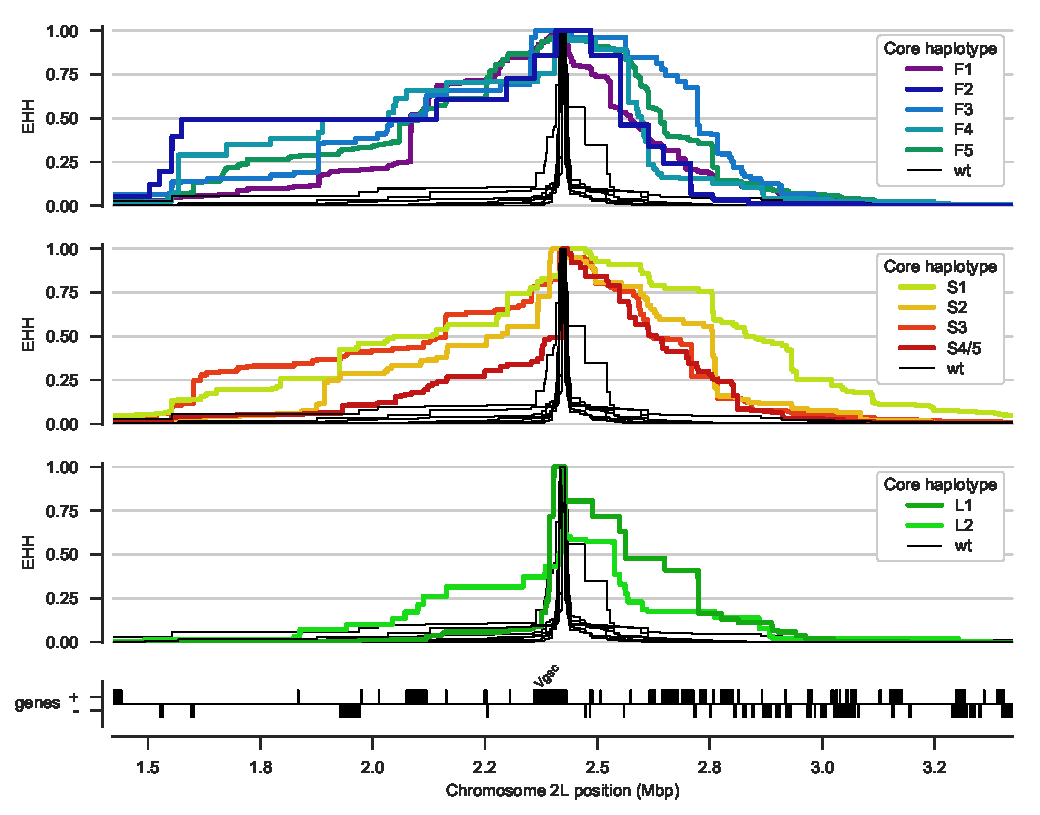
\includegraphics[width=1.1\linewidth,center]{artwork/ehh_decay.pdf}
  \caption{\textbf{Evidence for positive selection on haplotypes carrying known or putative resistance alleles}. Each panel plots the decay of extended haplotype homozygosity (EHH) for a set of core haplotypes centred on \textit{Vgsc} codon 995. Core haplotypes F1-F5 carry the \texttt{L995F} allele; S1-S4/5 carry the \texttt{L995S} allele; L1 carries the \texttt{I1527T} allele; L2 carries the \texttt{M490I} allele. Wild-type (wt) haplotypes do not carry any of these alleles. A slower decay of EHH relative to wild-type haplotypes implies positive selection (each panel plots the same collection of wild-type haplotypes).}
  \label{fig:ehh_decay}
\end{figure}
%%


%%
%
As expected, haplotypes carrying the \texttt{L995F} and \texttt{L995S} resistance alleles all experience a dramatically slower decay of EHH relative to wild-type haplotypes, confirming positive selection.
%
Previous studies have found evidence for different rates of EHH decay between \texttt{L995F} and \texttt{L995S} haplotypes, which could be due to differences in haplotype ages and/or selection coefficients.
%
However, we found no significant difference in EHH decay between these two alleles (@@TODO data).
%
The L1 haplotype carrying \texttt{I1527T+V402L} exhibited a slow decay of EHH on the downstream flank of the gene, similar to haplotypes carrying \texttt{L995F} and \texttt{L995S}, indicating that this combination of alleles has experienced positive selection.
%
EHH decay on the upstream gene flank was faster, being similar to wild-type haplotypes, however we know from the analyses described above that there is evidence for recombination between \texttt{I1527T} and \texttt{V402L} within this group of haplotypes, and thus a faster decay of EHH is expected upstream of the core locus. 
%
The L2 haplotype carrying \texttt{M490I} exhibited EHH decay intermediate between wild-type haplotypes and haplotypes carrying known resistance alleles.
%
This could indicate evidence for selection on the \texttt{M490I} allele, however these haplotypes are derived from a Kenyan mosquito population which is known to have experienced a severe recent bottleneck \cite{Ag1000gConsortium2017}, and there are no wild-type haplotypes from Kenya with which to compare, thus this signal may also be due to the extreme demographic history of this population.
%%


%%%%%%%%%%%%%%%%%%%%%%%%%%%%%%%%%%%%%%%%%%%%%%%%%%%%%%%%%%%%%%%%%%%%%%%%%%%%%%%
\subsection*{Design of genetic assays for surveillance of pyrethroid resistance}

%%
%
Entomological surveillance teams in Africa do regularly genotype mosquitoes for resistance alleles in \textit{Vgsc} codon 995, and use those results as an indicator for the presence of pyrethroid resistance alongside results from insecticide resistance bioassays.
%
They typically do not, however, sequence the gene or genotype any other polymorphisms within the gene.
%
Thus if there are other polymorphisms within the gene that cause or significantly enhance pyrethroid resistance, these will not be detected.
%
Also, if a codon 995 resistance allele is observed, there is no way to know whether the allele is on a genetic background that has also been observed in other mosquito populations, and thus no way to investigate whether resistance alleles are emerging locally or being imported from elsewhere, and if so, what is the probable source population.
%
Whole-genome sequencing clearly provides data of sufficient resolution to answer these questions, and portable genome sequencing will no doubt be feasible within the next few years.
%
However, in the interim it may be worthwhile to develop low-cost, high-throughput targeted genetic assays for surveillance of \textit{Vgsc}-mediated pyrethroid resistance.
%
For example, it would be feasible to design primers for amplicon sequencing, which could provide genotypes for of the order of 100 SNPs in a single amplicon panel, and could be implemented at low cost using existing sequencing platforms in regional sequencing facilities.
%%


%% Figure - Information gain.
%
\begin{figure}[!t]
  \centering
  
  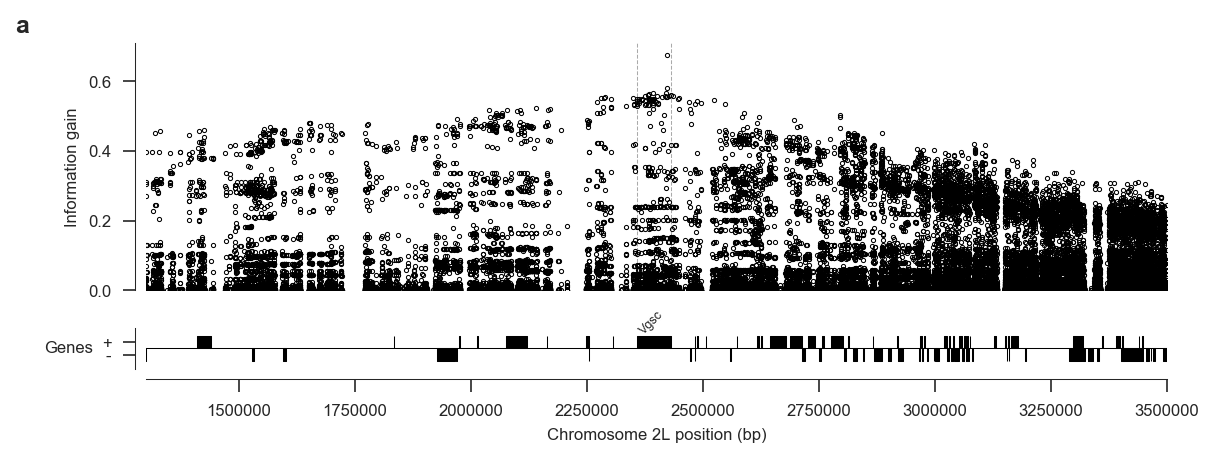
\includegraphics[width=1.0\linewidth]{artwork/info_gain.png}
  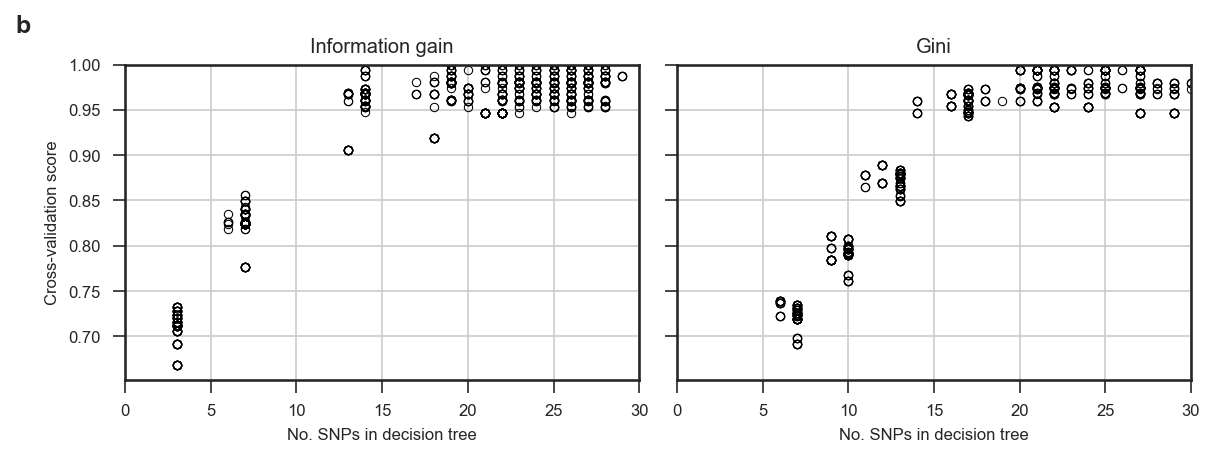
\includegraphics[width=1.0\linewidth]{artwork/tree_cv.png}
  
  \caption{%
%
\textbf{Informative SNPs for haplotype surveillance}. 
%
\textbf{a}, Each data point represents a single SNP. 
%
The information gain value for each SNP provides an indication of how informative the SNP is likely to be if used as part of a genetic assay for testing whether a mosquito carries a resistance haplotype, and if so, which of the known resistance haplotype clusters it derives from. 
%
\textbf{b}, Number of SNPs required to accurately classify which cluster a haplotype derives from. 
%
Decision trees were constructed using either the LD3 (left) or CART (right) algorithm for comparison.
%
Accuracy was evaluated using 10-fold stratified cross-validation.
}

  \label{fig:gain}
\end{figure}
%%

%%
%
To facilitate the development of targeted genetic assays for surveillance of \textit{Vgsc}-mediated pyrethroid resistance, we have produced two supplementary data tables.
%
In Supplementary Table 1 we provide a list of all @@N biallelic SNPs discovered with high confidence in the Ag1000G phase 1 cohort within the \textit{Vgsc} gene and in the 100 kbp upstream and downstream flanking regions.
%
To aid in PCR primer design, for each SNP we provide the flanking sequence for 250 bp upstream and downstream of the SNP position, including information about any polymorphisms within these flanking regions.
%
Not all SNPs are informative for detecting whether an individual mosquito carries a resistance allele, or diagnosing which genetic background is present, and we provide some summary statistics for each SNP to aid in the identification of the most informative SNPs.
%
This includes allele frequencies for each of the 10 haplotype clusters identified here as carrying known or probable resistance alleles, as well as for wild-type haplotypes from different locations.
%
To help with designing classifiers than can accurately call resistance haplotypes with a minimal number of SNPs, we also provide the information gain \cite{Quinlan1986} and the Gini impurity \cite{Breiman1984} for each SNP.
%
Note that recombination events are more likely at increasing distances upstream and downstream of the resistance variants under selection, and thus the most informative SNPs are found closest to the resistance variants within the gene (Figure \ref{fig:gain}).
%
However, SNPs with some information gain are available throughout the gene and in flanking regions.
%
%%

%%
%
A possible strategy for the design of a genetic assay could proceed by (1) performing an initial round of filtering to remove SNPs which are not informative (e.g., low information gain); (2) performing a round of primer design to remove SNPs for which primers are unlikely to be successful; (3) performing a full analysis of the remaining SNPs to select a subset that is sufficient to classify all resistance haplotypes identified here, including some redundancy; (4) finalise primer designs for the chosen panel of SNPs.
%
A possible methodology for step 3 would be to use an algorithm such as ID3 \cite{Quinlan1986} or CART \cite{Breiman1984} to build a decision tree, although many other algorithms for building classifiers are also applicable.
%
To aid in the development of a classifier, in Supplementary Table 2 we provide our classification for each of the 1530 haplotypes sampled here, along with the alleles carried by each haplotype for each of the SNPs included in Supplementary Table 1.
%
To test the methodology, we constructed decision trees using either LD3 or CART algorithms, and using all available SNPs from within the \textit{Vgsc} plus 20 kbp flanking regions as input features (i.e., assuming primers could be designed in all cases).
%
Figure \ref{fig:gain}b shows the cross-validation scores obtained for trees constructed allowing increasing numbers of SNPs.
%
This analysis suggests that it should be possible to construct a decision tree able to classify resistance haplotypes with >95\% accuracy using 20 SNPs or less.
%%




%%%%%%%%%%%%%%%%%%%%%%%%%%%%%%%%%%%%%%%%%%%%%%%%%%%%%%%%%%%%%%%%%%%%%%%%%%%%%%%
%%%%%%%%%%%%%%%%%%%%%%%%%%%%%%%%%%%%%%%%%%%%%%%%%%%%%%%%%%%%%%%%%%%%%%%%%%%%%%%
\section*{Discussion}
%%


%%%%%%%%%%%%%%%%%%%%%%%%%%%%%%%%%%%%%%%%%%%%%%%%%%%%%%%%%%%%%%%%%%%%%%%%%%%%%%%
\subsection*{Cross-resistance between pyrethroids and DDT}


%%
%
The VGSC protein is the physiological target of both pyrethroid insecticides and DDT @@REF.
%
The \texttt{L995F} and \texttt{L995S} alleles are known to increase resistance to both of these insecticide classes @@REF.
%
Except in a few locations, DDT has not been used for IRS within the last two decades, and is not suitable for use in bed-nets @@REF.
%
DDT was, however, used in Africa for several pilot IRS projects carried out during the first global campaign to eradicate malaria, during the 1950s and 1960s @@REF.
%
DDT was also used in agriculture throughout @@decades, and although agricultural usage has greatly diminished since @@decade, some usage may remain.
%
In this study we reported evidence of positive selection on haplotypes carrying \texttt{L995F} and haplotypes carrying \texttt{L995S}, as well as haplotypes carrying the \texttt{I1527T+V402L} combination.
%
We also found 14 other non-synonymous substitutions within \textit{Vgsc} that have arisen in association with \texttt{L995F} and appear to be positively selected.
%
Given that pyrethroids have dominated public health insecticide use for two decades, it is reasonable to assume that the selection pressure on these alleles is primarily due to pyrethroids.
%
If a resistance allele had been selected primarily by the earlier phase of DDT usage, then we might expect to see a faster rate of EHH decay for haplotypes carrying that allele relative to other alleles selected by recent pyrethroid usage.
%
However, we found no significant difference between EHH decay for haplotypes carrying \texttt{L995F} or \texttt{L995S} @@TODO confirm.
%
EHH decay was faster on the upstream flank for haplotypes carrying \texttt{I1527T}, however this may be affected by selection for the combination of \texttt{I1527T+V402L} and thus for recombination events that bring these two variants together on the same haplotype.
%
Nevertheless, it is possible that some if not all of the alleles we have reported provide some level of cross-resistance to DDT as well as pyrethroids, and that earlier DDT usage may have contributed at least in part to their selection.
%
%%


%%%%%%%%%%%%%%%%%%%%%%%%%%%%%%%%%%%%%%%%%%%%%%%%%%%%%%%%%%%%%%%%%%%%%%%%%%%%%%%
\subsection*{Prediction of resistance phenotypes for novel non-synonymous variants}

%%
%
...with the evidence for selection on Anopheles haplotypes, knowledge of the gene structure and evidence from other systems we can begin to predict resistance phenotypes for novel non-synonymous variants...
%%
See Table 2

@@TODO collect all material related to resistance phenotype prediction here, after we have results from analyses of selection.


%% Table 2 - Phenotype.
%
\afterpage{%
%\clearpage
% N.B., for some reason using \newgeometry causes page number to get dropped from the subsequent page, so disable for now - not needed if using \footnotesize.
%\newgeometry{margin=2cm}
\begin{landscape}
\thispagestyle{empty}
\begin{table}[h]
  \scriptsize
  \centering
  \begin{threeparttable}

  \caption{
%
\textbf{Phenotype prediction in the voltage-gated sodium channel gene}. 
}

  \label{table:variants_pheno}
  
  
\begin{tabular}{llllll}
\toprule
\multicolumn{2}{c}{Variant} &
\multicolumn{4}{c}{Function}\\
\cmidrule(r){1-2}
\cmidrule(r){3-6}
\emph{Ag} & 
\emph{Md} & Domain\tnote{1} & 
Predicted phenotype\tnote{2} &
Experimental evidence\tnote{3} &
Publication\\
\midrule

\texttt{R254K} & \texttt{R261} & \texttt{IN (I.S4--I.S5)} & \texttt{L995F} enhancer (predicted) & \texttt{L995F} enhancer (predicted) & \texttt{IN (I.S4--I.S5)} \\

\texttt{V402L} & \texttt{V410} & \texttt{TM (I.S6)} & \texttt{I1527T} enhancer (predicted) & \texttt{I1527T} enhancer (predicted) & \texttt{TM (I.S6)} \\

\texttt{V402L} & \texttt{V410} & \texttt{TM (I.S6)} & \texttt{I1527T} enhancer (predicted) & \texttt{I1527T} enhancer (predicted) & \texttt{TM (I.S6)} \\

\texttt{D466H} & \texttt{-} & \texttt{IN (I.S6--II.S1)} & \texttt{L995F} enhancer (predicted) & \texttt{L995F} enhancer (predicted) & \texttt{IN (I.S6--II.S1)} \\

\texttt{M490I} & \texttt{M508} & \texttt{IN (I.S6--II.S1)} & none (predicted) & none (predicted) & \texttt{IN (I.S6--II.S1)} \\

\texttt{M490I} & \texttt{M508} & \texttt{IN (I.S6--II.S1)} & none (predicted) & none (predicted) & \texttt{IN (I.S6--II.S1)} \\

\texttt{T791M} & \texttt{T810} & \texttt{TM (II.S1)} & \texttt{L995F} enhancer (predicted) & \texttt{L995F} enhancer (predicted) & \texttt{TM (II.S1)} \\

\texttt{L995S} & \texttt{L1014} & \texttt{TM (II.S6)} & driver & driver & \texttt{TM (II.S6)} \\

\texttt{L995F} & \texttt{L1014} & \texttt{TM (II.S6)} & driver & driver & \texttt{TM (II.S6)} \\

\texttt{A1125V} & \texttt{K1133} & \texttt{IN (II.S6--III.S1)} & none (predicted) & none (predicted) & \texttt{IN (II.S6--III.S1)} \\

\texttt{V1254I} & \texttt{I1262} & \texttt{IN (II.S6--III.S1)} & none (predicted) & none (predicted) & \texttt{IN (II.S6--III.S1)} \\

\texttt{I1527T} & \texttt{I1532} & \texttt{TM (III.S6)} & driver (predicted) & driver (predicted) & \texttt{TM (III.S6)} \\

\texttt{N1570Y} & \texttt{N1575} & \texttt{IN (III.S6--IV.S1)} & \texttt{L995F} enhancer & \texttt{L995F} enhancer & \texttt{IN (III.S6--IV.S1)} \\

\texttt{E1597G} & \texttt{E1602} & \texttt{IN (III.S6--IV.S1)} & \texttt{L995F} enhancer (predicted) & \texttt{L995F} enhancer (predicted) & \texttt{IN (III.S6--IV.S1)} \\

\texttt{K1603T} & \texttt{K1608} & \texttt{TM (IV.S1)} & \texttt{L995F} enhancer (predicted) & \texttt{L995F} enhancer (predicted) & \texttt{TM (IV.S1)} \\

\texttt{A1746S} & \texttt{A1751} & \texttt{TM (IV.S5)} & \texttt{L995F} enhancer (predicted) & \texttt{L995F} enhancer (predicted) & \texttt{TM (IV.S5)} \\

\texttt{V1853I} & \texttt{V1858} & \texttt{IN (IV.S6--)} & \texttt{L995F} enhancer (predicted) & \texttt{L995F} enhancer (predicted) & \texttt{IN (IV.S6--)} \\

\texttt{I1868T} & \texttt{I1873} & \texttt{IN (IV.S6--)} & \texttt{L995F} enhancer (predicted) & \texttt{L995F} enhancer (predicted) & \texttt{IN (IV.S6--)} \\

\texttt{P1874S} & \texttt{P1879} & \texttt{IN (IV.S6--)} & \texttt{L995F} enhancer (predicted) & \texttt{L995F} enhancer (predicted) & \texttt{IN (IV.S6--)} \\

\texttt{P1874L} & \texttt{P1879} & \texttt{IN (IV.S6--)} & \texttt{L995F} enhancer (predicted) & \texttt{L995F} enhancer (predicted) & \texttt{IN (IV.S6--)} \\

\texttt{F1920S} & \texttt{Y1925} & \texttt{IN (IV.S6--)} & \texttt{L995F} enhancer (predicted) & \texttt{L995F} enhancer (predicted) & \texttt{IN (IV.S6--)} \\

\texttt{A1934V} & \texttt{A1939} & \texttt{IN (IV.S6--)} & \texttt{L995F} enhancer (predicted) & \texttt{L995F} enhancer (predicted) & \texttt{IN (IV.S6--)} \\

\texttt{I1940T} & \texttt{I1945} & \texttt{IN (IV.S6--)} & \texttt{L995F} enhancer (predicted) & \texttt{L995F} enhancer (predicted) & \texttt{IN (IV.S6--)} \\

\bottomrule
\end{tabular}

  
  \begin{tablenotes}
    \footnotesize
    
    \item[1] Position of the variant within the protein. \texttt{IN}=internal domain; \texttt{TM}=trans-membrane domain. The protein contains four homologous repeats (I-IV), each having six transmembrane segments (1-6). Codes in parentheses identify the specific domain, e.g., ``\texttt{I.S4}'' refers to trans-membrane segment 4 in repeat I, and ``\texttt{IS4--IS5}'' refers to the linker segment between \texttt{I.S4} and \texttt{I.S5}.
    
    \item[2] Phenotype predictions are based on population genetic evidence and have not been confirmed experimentally.
    
    \item[3] Literature search results for experimental evidence, assoc. - association study, \emph{in vitro} - \emph{Xenopus} oocytes.
    
    \item[4] Publication from which evidence is taken.
    
  \end{tablenotes}
  
  \end{threeparttable}
  
\end{table}
\end{landscape}
%\restoregeometry
} % end afterpage
%% end Table 2



@@TODO


\section*{Legacy Discussion Points/ Discussion Sandbox}
%%


@@TODO HW disequilibrium in Gabon - what might be happening here?

@@TODO Discuss accessibility, have we missed any functional variation?

@@TODO Speculate on why \texttt{L995F} but not \texttt{L995S} has evolved secondary variation.

@@TODO What about DDT? If prior selection for DDT resistance, how might this complicate the picture? Do we see any evidence for multiple phases of selection?

@@TODO Discuss weaknesses, caveats and potential improvements to method for estimating haplotype age.

@@TODO What are the implications for insecticide resistance management? Realistically how could this information be used?


%%%%%%%%%%%%%%%%%%%%%%%%%%%%%%%%%%%%%%%%%%%%%%%%%%%%%%%%%%%%%%%%%%%%%%%%%%%%%%%
\subsection*{Assay design discussion}
%%
The insecticide resistance driven selective sweeps we have identified here are likely ongoing, affecting many more mosquito populations than we have sampled in Ag1000G phase 1, and continuing to spread.
%
In addition, other selective events may be occurring in populations that we have not sampled, or in populations we have sampled but since the sampling date.
%
Whole-genome sequencing of individual mosquitoes clearly provides data of sufficient resolution to identify resistance sweeps, and could also be used to provide ongoing resistance surveillance.
%
The cost of whole-genome sequencing continues to fall, with the present cost being approximately 100 GBP to obtain \textasciitilde$30\times$ coverage of an individual \emph{Anopheles} mosquito genome with 150 bp paired-end reads.
%
Mobile sequencing using nanopore technology is also developing rapidly \cite{Jain2016} and may be a realistic prospect for mosquito whole-genome sequencing within a few years.
%
There is an interim period, however, during which it may be more practical to develop targeted genetic assays for outbreak surveillance that could scale to tens of thousands of mosquitoes at low cost.
%
For example, both next-generation and mobile sequencing platforms can be used for amplicon sequencing, where specific genome regions are amplified and sequenced in highly multiplexed libraries \cite{Bybee2011, Murray2015}.
%
Our results show that during this interim it is possible to quickly produce assays to cheaply allow tracking of putative resistant bearing haplotypes, in real time, in the field.
%%




%%%%%%%%%%%%%%%%%%%%%%%%%%%%%%%%%%%%%%%%%%%%%%%%%%%%%%%%%%%%%%%%%%%%%%%%%%%%%%%
%%%%%%%%%%%%%%%%%%%%%%%%%%%%%%%%%%%%%%%%%%%%%%%%%%%%%%%%%%%%%%%%%%%%%%%%%%%%%%%
\section*{Methods}


%%%%%%%%%%%%%%%%%%%%%%%%%%%%%%%%%%%%%%%%%%%%%%%%%%%%%%%%%%%%%%%%%%%%%%%%%%%%%%%
\subsection*{Code}

%
All scripts and Jupyter Notebooks used to generate analyses, figures and tables are available from the GitHub repository \url{https://github.com/malariagen/agam-vgsc-report}. 
%%


%%%%%%%%%%%%%%%%%%%%%%%%%%%%%%%%%%%%%%%%%%%%%%%%%%%%%%%%%%%%%%%%%%%%%%%%%%%%%%%
\subsection*{Data}

%
We used variant call data from the phase 1 AR3 release and phased haplotype data from AR3.1. These data are publically downloadable via ftp from \url{https://www.malariagen.net}. 
%
@@add ENA from paper
%%


%%%%%%%%%%%%%%%%%%%%%%%%%%%%%%%%%%%%%%%%%%%%%%%%%%%%%%%%%%%%%%%%%%%%%%%%%%%%%%%
\subsection*{Data collection and processing}

%
For detailed information on Ag1000g WGS sample collection, sequencing, variant calling, quality control and phasing see \cite{Ag1000gConsortium2017}.
%
In brief, \emph{An. gambiae} and \emph{An. coluzzii} mosquitoes were collected from eight countries across Sub-Saharan Africa: Angola, Burkina Faso, Cameroon, Gabon, Guinea, Guinea Bissau, Kenya and Uganda. 
%
From Angola just \emph{An. coluzzii} were sampled, Burkina Faso had samples of both \emph{An. gambiae} and \emph{An. coluzzii} and all other populations consisted of purely \emph{An. gambiae} except for Kenya and Guinea Bissau, where species status is uncertain \cite{Ag1000gConsortium2017}.
%
Mosquitoes were individually whole genome sequenced on the Illumina HiSeq 2000 platform, generating 100bp paired-end reads. 
%
Sequenced reads were aligned to the \cite{An. gambiae} AgamP3 reference genome assembly \cite{Holt2002}). 
%
Aligned bam files underwent improvement, before variants were called using GATK UnifiedGenotyper. 
%
Quality control included removal of samples with mean coverage <= 14x and an accessibility map was employed following a similar approach to that used for human data by The 1000 Genomes Project Consortium \cite{The1000GenomesProjectConsortium2010}). 
%
Various quality control filters were applied to remove samples and SNPs with poor quality data. 
%
This process produced a call set containing @@n SNPs genotyped in 765 wild-caught individual mosquitoes \cite{Ag1000gConsortium2017}.
%%

%
The Ag1000g variant data was functionally annotated using the SnpEff v4.1b software which allowed investigation of potential phenotype altering variants within \emph{Vgsc} \cite{Cingolani2012}.
%
Non-synonymous \emph{Vgsc} variants were identified as all variants in AGAP004707, 2L:2358158-2431617, with a SnpEff annotation of “missense”  and an ALT allele frequency of >5\% in at least one of the nine mosquito populations, with the exceptions of the multi-allelic SNP 2L:2400071 G>A which is shown despite only being found in \emph{An. gambiae} from Cameroon at 0.4\% frequency, as the G>T variant at the same position which causes the same codon change (\texttt{M490I}), is found above 5\% frequency in Kenya.
%
\texttt{F1920S} is included for continuity with recent \emph{An. gambiae Vgsc} research \cite{Ag1000gConsortium2017}.
%
A minimum ALT allele frequency was employed to discriminate towards variants that may be undergoing selective sweeps and against less informative low frequency alleles.
%%

%
For ease of comparison with previous work on \emph{Vgsc}, pan Insecta, in Table \ref{table:variants_missense} we report codon numbering for both \emph{An. gambiae} and \emph{Musca domestica} (the species in which the gene was first discovered).
%
The \emph{M. domestica Vgsc} sequence (EMBL accession X96668 - \cite{Williamson1996}) was aligned with the \emph{An. gambiae} AGAP004707-RA sequence (AgamP4.4 gene-set), using the Mega v7 software package \cite{Kumar2016}.
%
A map of equivalent codon numbers between the two species can be download from the MalariaGEN website (@@include as supplementary data file?)- 
\url{https://www.malariagen.net/sites/default/files/content/blogs/domestica_gambiae_map.txt}.
%%

%
Haplotypes for each chromosome of each sample were estimated (phased) using using phase informative reads (PIRs) and SHAPEIT2 v2.r837 \cite{Delaneau2013}, see \cite{Ag1000gConsortium2017} supplementary text for more details.
%
The SHAPEIT2 algorithm is unable to phase multi-allelic positions, therefore the two multi-allelic non-synonymous SNPs within the \emph{Vgsc} gene (>5\% ALT frequency in at least one population), altering codons \texttt{V402} and \texttt{M490}, were phased onto the haplotypes using MVNcall v1.0 \cite{Menelaou2013}.
%
Conservative filtering had removed one of the three known insecticide resistance conferring kdr variants, \texttt{N1570Y} \cite{Jones2012}.
%
After manual inspection of the read alignment revealed that the SNP call could be confidently made, it was added back into the data set and then also phased onto the haplotypes using MVNcall.
%
To evaluate the linkage disequilibrium (LD) of non-synonymous \emph{Vgsc} mutations with the two most widespread \emph{kdr} resistance mutations (\texttt{L995S/F}), the D1 statistic was calculated using haplotypes.
%%


%%%%%%%%%%%%%%%%%%%%%%%%%%%%%%%%%%%%%%%%%%%%%%%%%%%%%%%%%%%%%%%%%%%%%%%%%%%%%%%
\subsection*{Haplotype networks}

%
Discerning the relationships between similar haplotypes can be difficult when using bifurcating trees as, inherently, the distance between the leaves at the tips (haplotypes) will be small.
%
As these relationships may be informative of the history of selection, we utilised a network approach to elucidate them.
%
We constructed haplotype networks using the median-joining algorithm \cite{Bandelt1999} as implemented in a custom Python script available from \url{https://github.com/malariagen/agam-vgsc-report}.
%
Haplotypes carrying either \texttt{L995F} or \texttt{L995S} mutations were analysed with a maximum edge distance of two SNPs, to ensure networks contained haplotypes with recent common ancestors.
%
Networks were rendered with the graphviz library and a composite figure constructed using Inkscape.
%
Non-synonymous edges were highlighted using the SnpEff annotations \cite{Cingolani2012}.
%%


%%%%%%%%%%%%%%%%%%%%%%%%%%%%%%%%%%%%%%%%%%%%%%%%%%%%%%%%%%%%%%%%%%%%%%%%%%%%%%%
\subsection*{IBD}

%
IBD. @@TODO - AM
-Length of shared haplotype and number of mutations between them are informative of age…
-Pairwise t values were hierarchically clustered and visualised as a dendrogram using the Python library Scipy and its cluster hierarchy functions linkage method.
-Cutting the dendrogram at @@generations clustered haplotypes together into haplogroups…
- Naming of haplogroups with reference to Ag1000g...
-dendro figure/distro figures/map - Python libraries...
%%


%%%%%%%%%%%%%%%%%%%%%%%%%%%%%%%%%%%%%%%%%%%%%%%%%%%%%%%%%%%%%%%%%%%%%%%%%%%%%%%
\subsection*{Recombination}

%
EHH @@TODO AM
%%


%%%%%%%%%%%%%%%%%%%%%%%%%%%%%%%%%%%%%%%%%%%%%%%%%%%%%%%%%%%%%%%%%%%%%%%%%%%%%%%
\subsection*{Recombination}

%
Recombination. @@TODO - AM - Absolute divergence dxy...
%%


%%%%%%%%%%%%%%%%%%%%%%%%%%%%%%%%%%%%%%%%%%%%%%%%%%%%%%%%%%%%%%%%%%%%%%%%%%%%%%%
\subsection*{Haplotype tagging SNPs}

%
Tagging SNPs. @@TODO - AM
%%



%%%%%%%%%%%%%%%%%%%%%%%%%%%%%%%%%%%%%%%%%%%%%%%%%%%%%%%%%%%%%%%%%%%%%%%%%%%%%%%
%%%%%%%%%%%%%%%%%%%%%%%%%%%%%%%%%%%%%%%%%%%%%%%%%%%%%%%%%%%%%%%%%%%%%%%%%%%%%%%
\printbibliography


\beginsupplement
%%%%%%%%%%%%%%%%%%%%%%%%%%%%%%%%%%%%%%%%%%%%%%%%%%%%%%%%%%%%%%%%%%%%%%%%%%%%%%%
%%%%%%%%%%%%%%%%%%%%%%%%%%%%%%%%%%%%%%%%%%%%%%%%%%%%%%%%%%%%%%%%%%%%%%%%%%%%%%%
\section*{Supplementary figures}


\clearpage

%% Figure - L995F recombination
%
\begin{figure}[!t]
  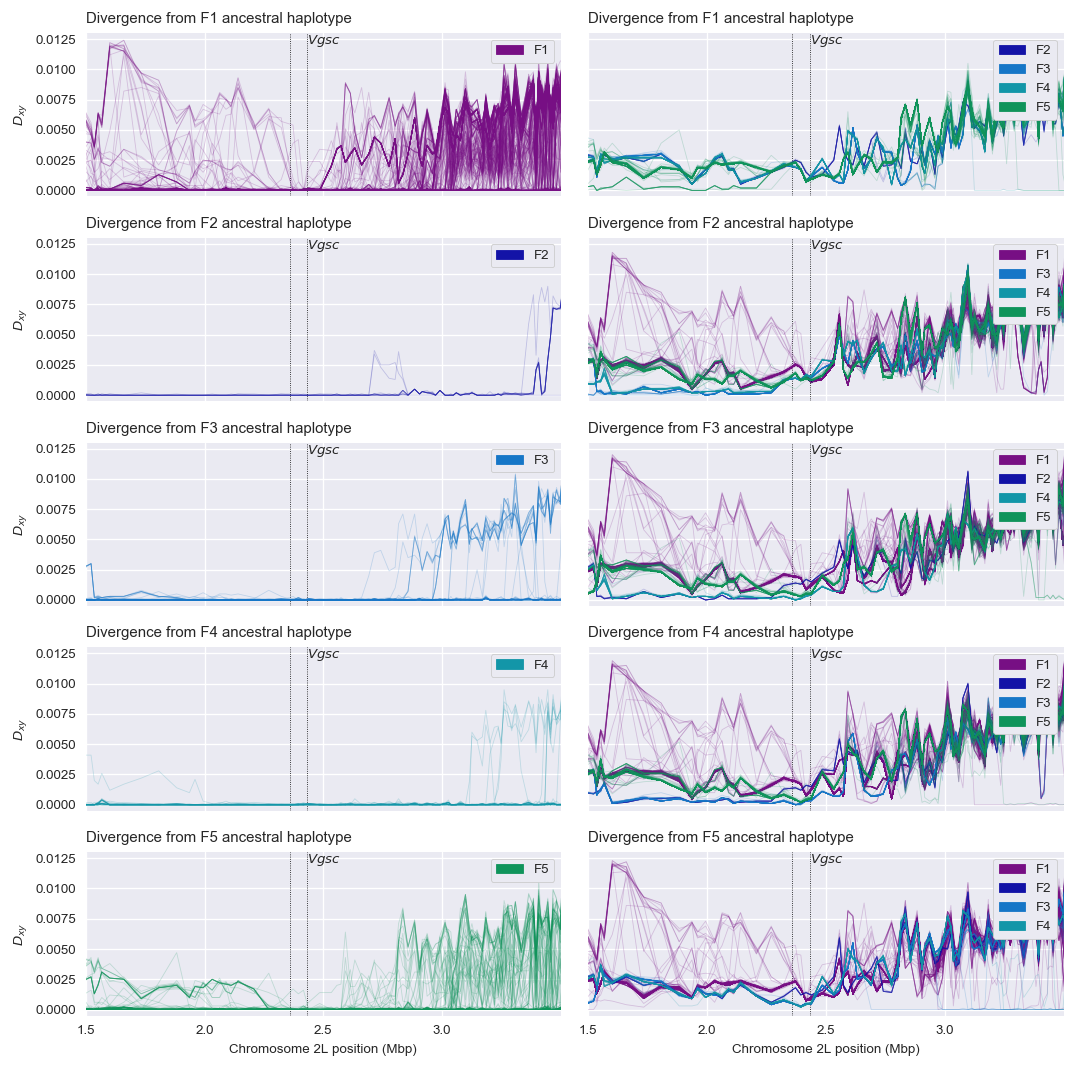
\includegraphics[width=1.1\linewidth,center]{artwork/fig_recom_F.png}
  \caption{\textbf{Moving window analysis of genetic distance between haplotypes carrying the \texttt{L995F} allele}. Panels on the left plot the divergence of haplotypes within a haplotype cluster, relative to an inferred ancestral haplotype. Panels on the right plot divergence of haplotypes between different haplotype clusters. If haplotype clusters are unrelated (i.e., do not share a recent common ancestor) then divergence should be greater than zero within \textit{Vgsc} and flanking regions.}
  \label{fig:recom_f}
\end{figure}
%%

\clearpage

%% Figure - L995S recombination
%
\begin{figure}[!t]
  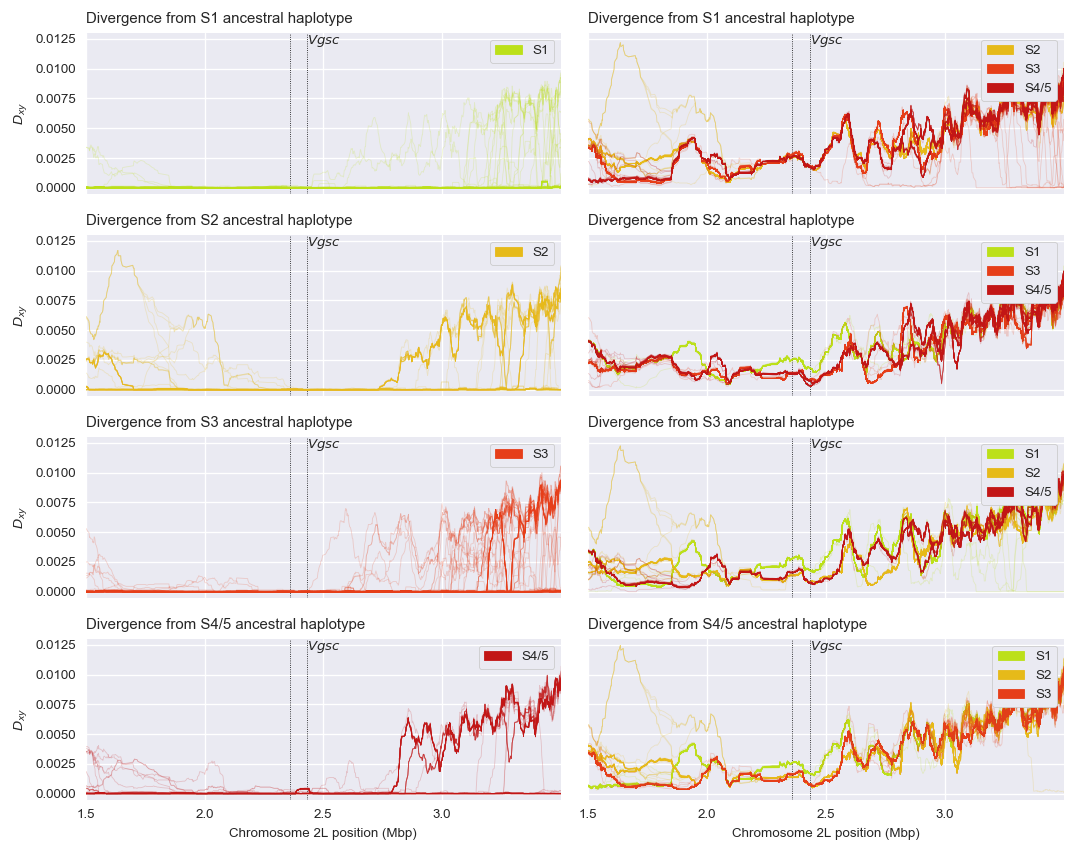
\includegraphics[width=1.1\linewidth,center]{artwork/fig_recom_S.png}
  \caption{\textbf{Moving window analysis of genetic distance between haplotypes carrying the \texttt{L995S} allele}. See Figure \ref{fig:recom_f} for explanation.}
  \label{fig:recom_s}
\end{figure}
%%


\clearpage

%% Figure - L995L recombination
%
\begin{figure}[!t]
  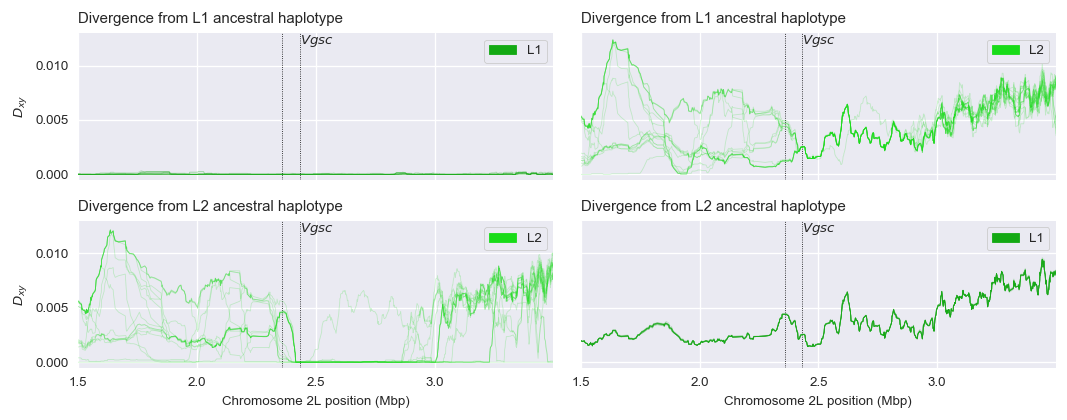
\includegraphics[width=1.1\linewidth,center]{artwork/fig_recom_L.png}
  \caption{\textbf{Moving window analysis of genetic distance between haplotypes carrying the \texttt{L995} allele}. See Figure \ref{fig:recom_f} for explanation.}
  \label{fig:recom_l}
\end{figure}
%%


\clearpage

%% Figure - Overall haplotype age distribution.
%
\begin{figure}[!t]
  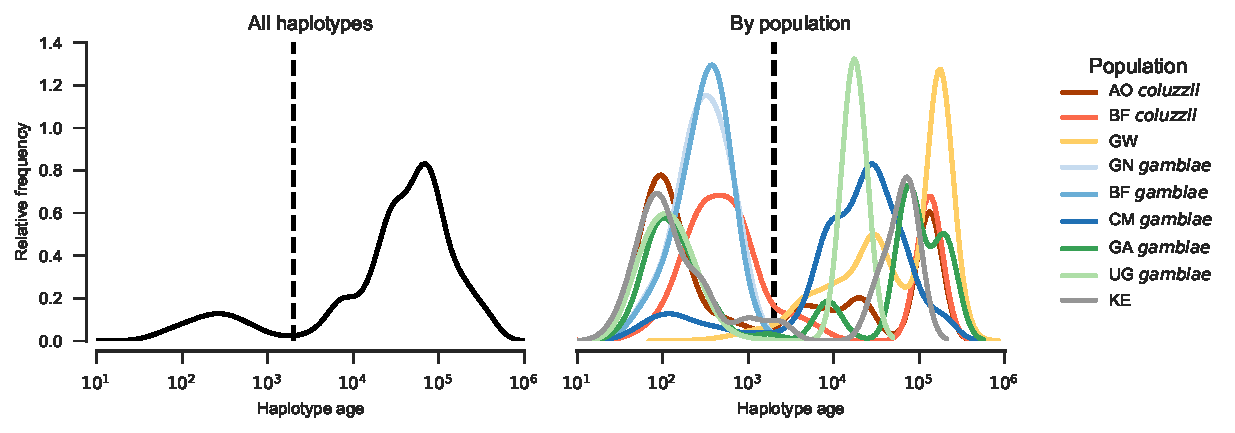
\includegraphics[width=1.1\linewidth,center]{artwork/haplotype_age_dist.pdf}
  \caption{\textbf{Distribution of pairwise haplotype ages estimated from IBD tract lengths spanning \textit{Vgsc}}. The left panel plots the distribution of ages between all haplotype pairs. The right panel plots ages for pairs within populations. Note that distributions are bimodal, implying that some haplotype pairs share a recent common ancestor while others share a common ancestor in the more distant past, expected if a selective sweep has occurred within the population. The vertical dashed line shows an approximate midpoint between the two modes.}
  \label{fig:age_hist}
\end{figure}
%%
 

\clearpage
 
%% Figure - Haplotype age tree.
%
\begin{figure}[!t]
  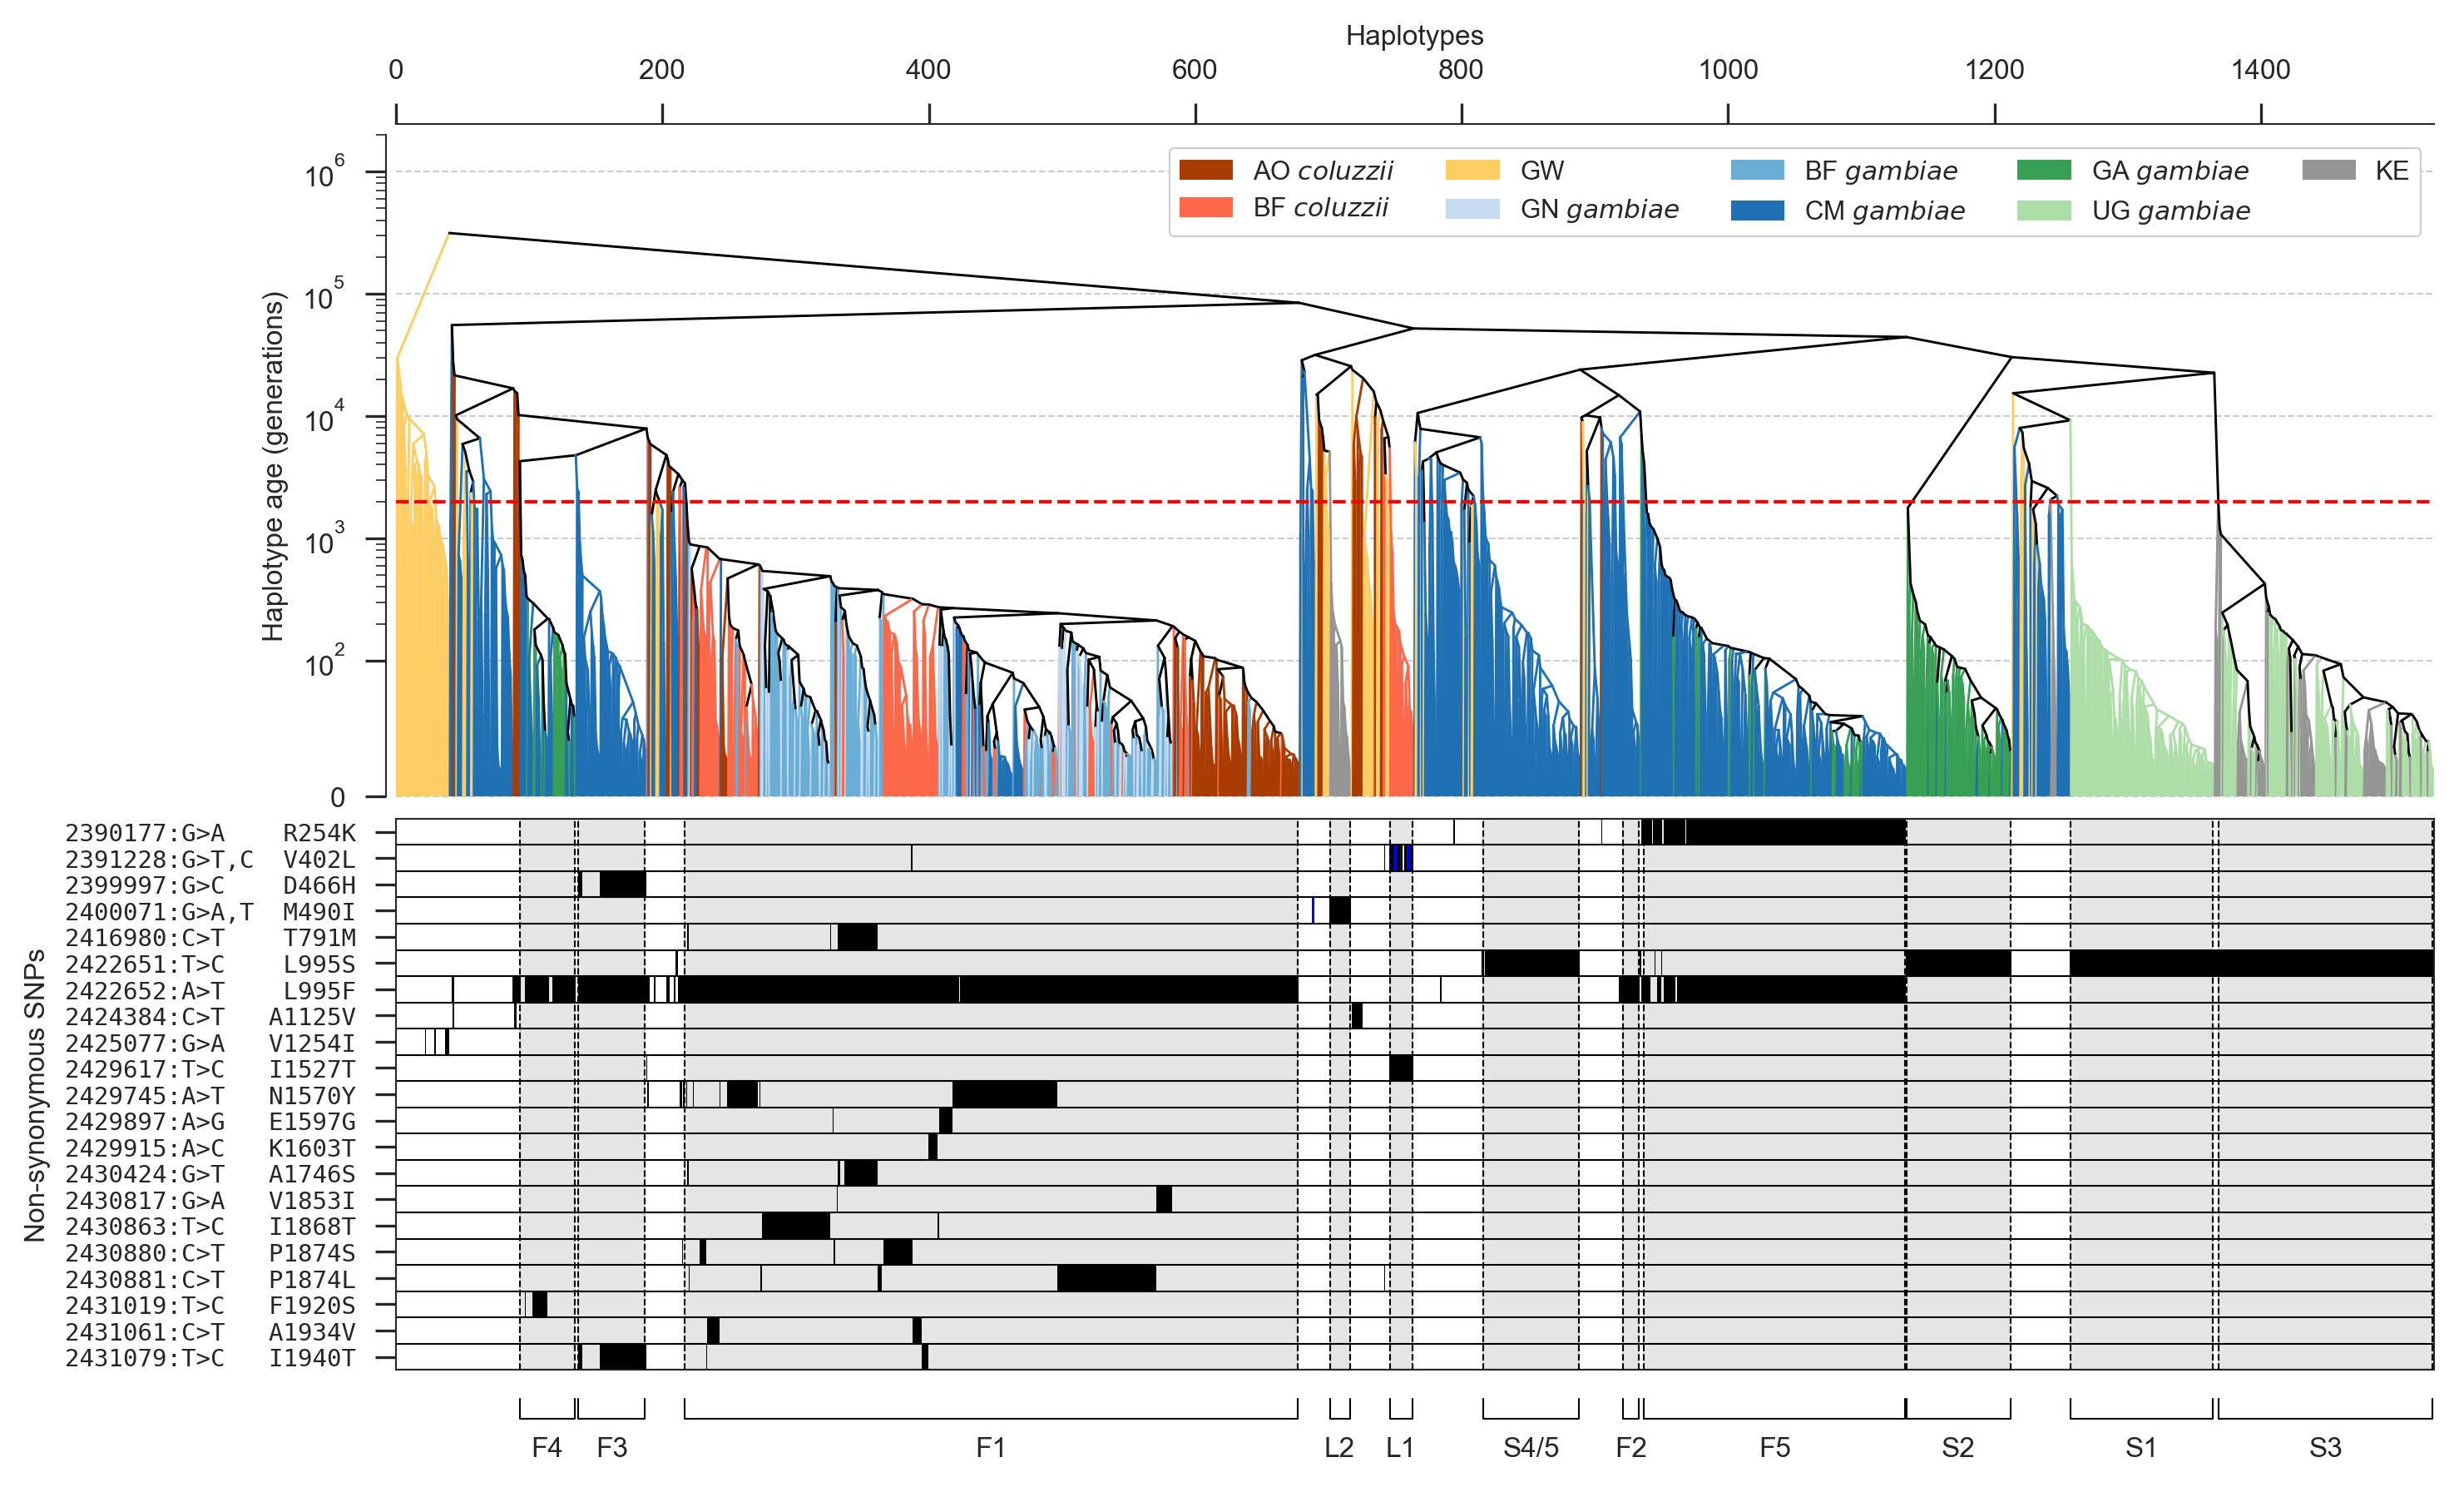
\includegraphics[width=1.1\linewidth,center]{artwork/fig_hap_tree.png}
  \caption{\textbf{Clustering of haplotypes by IBD tract lengths spanning \textit{Vgsc}}. @@TODO explain}
  \label{fig:tree}
\end{figure}
%%


\end{document}
